\documentclass[twoside]{book}

% Packages required by doxygen
\usepackage{calc}
\usepackage{doxygen}
\usepackage{graphicx}
\usepackage[utf8]{inputenc}
\usepackage{makeidx}
\usepackage{multicol}
\usepackage{multirow}
\PassOptionsToPackage{warn}{textcomp}
\usepackage{textcomp}
\usepackage[nointegrals]{wasysym}
\usepackage[table]{xcolor}

% Font selection
\usepackage[T1]{fontenc}
\usepackage{mathptmx}
\usepackage[scaled=.90]{helvet}
\usepackage{courier}
\usepackage{amssymb}
\usepackage{sectsty}
\renewcommand{\familydefault}{\sfdefault}
\allsectionsfont{%
  \fontseries{bc}\selectfont%
  \color{darkgray}%
}
\renewcommand{\DoxyLabelFont}{%
  \fontseries{bc}\selectfont%
  \color{darkgray}%
}
\newcommand{\+}{\discretionary{\mbox{\scriptsize$\hookleftarrow$}}{}{}}

% Page & text layout
\usepackage{geometry}
\geometry{%
  a4paper,%
  top=2.5cm,%
  bottom=2.5cm,%
  left=2.5cm,%
  right=2.5cm%
}
\tolerance=750
\hfuzz=15pt
\hbadness=750
\setlength{\emergencystretch}{15pt}
\setlength{\parindent}{0cm}
\setlength{\parskip}{0.2cm}
\makeatletter
\renewcommand{\paragraph}{%
  \@startsection{paragraph}{4}{0ex}{-1.0ex}{1.0ex}{%
    \normalfont\normalsize\bfseries\SS@parafont%
  }%
}
\renewcommand{\subparagraph}{%
  \@startsection{subparagraph}{5}{0ex}{-1.0ex}{1.0ex}{%
    \normalfont\normalsize\bfseries\SS@subparafont%
  }%
}
\makeatother

% Headers & footers
\usepackage{fancyhdr}
\pagestyle{fancyplain}
\fancyhead[LE]{\fancyplain{}{\bfseries\thepage}}
\fancyhead[CE]{\fancyplain{}{}}
\fancyhead[RE]{\fancyplain{}{\bfseries\leftmark}}
\fancyhead[LO]{\fancyplain{}{\bfseries\rightmark}}
\fancyhead[CO]{\fancyplain{}{}}
\fancyhead[RO]{\fancyplain{}{\bfseries\thepage}}
\fancyfoot[LE]{\fancyplain{}{}}
\fancyfoot[CE]{\fancyplain{}{}}
\fancyfoot[RE]{\fancyplain{}{\bfseries\scriptsize Generated on Thu Mar 27 2014 21\+:15\+:56 for Lib\+O\+P\+F\+::\+Plus by Doxygen }}
\fancyfoot[LO]{\fancyplain{}{\bfseries\scriptsize Generated on Thu Mar 27 2014 21\+:15\+:56 for Lib\+O\+P\+F\+::\+Plus by Doxygen }}
\fancyfoot[CO]{\fancyplain{}{}}
\fancyfoot[RO]{\fancyplain{}{}}
\renewcommand{\footrulewidth}{0.4pt}
\renewcommand{\chaptermark}[1]{%
  \markboth{#1}{}%
}
\renewcommand{\sectionmark}[1]{%
  \markright{\thesection\ #1}%
}

% Indices & bibliography
\usepackage{natbib}
\usepackage[titles]{tocloft}
\setcounter{tocdepth}{3}
\setcounter{secnumdepth}{5}
\makeindex

% Hyperlinks (required, but should be loaded last)
\usepackage{ifpdf}
\ifpdf
  \usepackage[pdftex,pagebackref=true]{hyperref}
\else
  \usepackage[ps2pdf,pagebackref=true]{hyperref}
\fi
\hypersetup{%
  colorlinks=true,%
  linkcolor=blue,%
  citecolor=blue,%
  unicode%
}

% Custom commands
\newcommand{\clearemptydoublepage}{%
  \newpage{\pagestyle{empty}\cleardoublepage}%
}


%===== C O N T E N T S =====

\begin{document}

% Titlepage & ToC
\hypersetup{pageanchor=false,
             bookmarks=true,
             bookmarksnumbered=true,
             pdfencoding=unicode
            }
\pagenumbering{roman}
\begin{titlepage}
\vspace*{7cm}
\begin{center}%
{\Large Lib\+O\+P\+F\+:\+:Plus }\\
\vspace*{1cm}
{\large Generated by Doxygen 1.8.6}\\
\vspace*{0.5cm}
{\small Thu Mar 27 2014 21:15:56}\\
\end{center}
\end{titlepage}
\clearemptydoublepage
\tableofcontents
\clearemptydoublepage
\pagenumbering{arabic}
\hypersetup{pageanchor=true}

%--- Begin generated contents ---
\chapter{libopf-\/plus}
\label{md_README}
\hypertarget{md_README}{}
An implementation of the Lib\+O\+P\+F Lib\+O\+P\+F developed in C++, taking all the advantages of oriented object design. 
\chapter{Test List}
\label{test}
\hypertarget{test}{}

\begin{DoxyRefList}
\item[\label{test__test000001}%
\hypertarget{test__test000001}{}%
Member \hyperlink{classopf_1_1ClassifyingStrategy_a7e41e0eca08359eb71653f42ab127241}{opf\+:\+:Classifying\+Strategy\+:\+:classify} (Model model, Patterns test)]test set of patterns. \begin{DoxySeeAlso}{See Also}
O\+P\+F\+Classifying 
\end{DoxySeeAlso}

\end{DoxyRefList}
\chapter{Namespace Index}
\section{Namespace List}
Here is a list of all namespaces with brief descriptions\+:\begin{DoxyCompactList}
\item\contentsline{section}{\hyperlink{namespaceopf}{opf} }{\pageref{namespaceopf}}{}
\end{DoxyCompactList}

\chapter{Hierarchical Index}
\section{Class Hierarchy}
This inheritance list is sorted roughly, but not completely, alphabetically\+:\begin{DoxyCompactList}
\item \contentsline{section}{Classifier}{\pageref{classClassifier}}{}
\item \contentsline{section}{Classifying\+Strategy}{\pageref{classClassifyingStrategy}}{}
\begin{DoxyCompactList}
\item \contentsline{section}{O\+P\+F\+Classifying}{\pageref{classOPFClassifying}}{}
\end{DoxyCompactList}
\item \contentsline{section}{Csv\+Adapter}{\pageref{classCsvAdapter}}{}
\item \contentsline{section}{Max\+Policy}{\pageref{classMaxPolicy}}{}
\item \contentsline{section}{Min\+Policy}{\pageref{classMinPolicy}}{}
\item \contentsline{section}{Model}{\pageref{classModel}}{}
\item \contentsline{section}{O\+P\+F}{\pageref{classOPF}}{}
\item \contentsline{section}{Pattern}{\pageref{classPattern}}{}
\item \contentsline{section}{Patterns}{\pageref{classPatterns}}{}
\item \contentsline{section}{Priority\+Queue}{\pageref{classPriorityQueue}}{}
\item \contentsline{section}{Prototypes\+Strategy}{\pageref{classPrototypesStrategy}}{}
\begin{DoxyCompactList}
\item \contentsline{section}{M\+S\+T\+Prototypes}{\pageref{classMSTPrototypes}}{}
\end{DoxyCompactList}
\item \contentsline{section}{Trainer}{\pageref{classTrainer}}{}
\item \contentsline{section}{Training\+Strategy}{\pageref{classTrainingStrategy}}{}
\begin{DoxyCompactList}
\item \contentsline{section}{O\+P\+F\+Training}{\pageref{classOPFTraining}}{}
\end{DoxyCompactList}
\end{DoxyCompactList}

\chapter{Class Index}
\section{Class List}
Here are the classes, structs, unions and interfaces with brief descriptions\+:\begin{DoxyCompactList}
\item\contentsline{section}{\hyperlink{classClassifier}{Classifier} }{\pageref{classClassifier}}{}
\item\contentsline{section}{\hyperlink{classClassifyingStrategy}{Classifying\+Strategy} \\*Interface for classifying strategies }{\pageref{classClassifyingStrategy}}{}
\item\contentsline{section}{\hyperlink{classCsvAdapter}{Csv\+Adapter} }{\pageref{classCsvAdapter}}{}
\item\contentsline{section}{\hyperlink{classMaxPolicy}{Max\+Policy} }{\pageref{classMaxPolicy}}{}
\item\contentsline{section}{\hyperlink{classMinPolicy}{Min\+Policy} }{\pageref{classMinPolicy}}{}
\item\contentsline{section}{\hyperlink{classModel}{Model} \\*Class for handling the training model informations }{\pageref{classModel}}{}
\item\contentsline{section}{\hyperlink{classMSTPrototypes}{M\+S\+T\+Prototypes} \\*Class to handle prototypes selection by using a Minimum Spanning Tree (M\+S\+T) }{\pageref{classMSTPrototypes}}{}
\item\contentsline{section}{\hyperlink{classOPF}{O\+P\+F} }{\pageref{classOPF}}{}
\item\contentsline{section}{\hyperlink{classOPFClassifying}{O\+P\+F\+Classifying} \\*Class to handle prototypes selection by using a Minimum Spanning Tree (M\+S\+T) }{\pageref{classOPFClassifying}}{}
\item\contentsline{section}{\hyperlink{classOPFTraining}{O\+P\+F\+Training} }{\pageref{classOPFTraining}}{}
\item\contentsline{section}{\hyperlink{classPattern}{Pattern} \\*Class for handling a single pattern }{\pageref{classPattern}}{}
\item\contentsline{section}{\hyperlink{classPatterns}{Patterns} \\*Class for handling a set of patterns }{\pageref{classPatterns}}{}
\item\contentsline{section}{\hyperlink{classPriorityQueue}{Priority\+Queue} \\*A class for handling minimum and maximum priority queues }{\pageref{classPriorityQueue}}{}
\item\contentsline{section}{\hyperlink{classPrototypesStrategy}{Prototypes\+Strategy} \\*Strategy interface of way to select prototypes }{\pageref{classPrototypesStrategy}}{}
\item\contentsline{section}{\hyperlink{classTrainer}{Trainer} }{\pageref{classTrainer}}{}
\item\contentsline{section}{\hyperlink{classTrainingStrategy}{Training\+Strategy} \\*Interface for training strategies }{\pageref{classTrainingStrategy}}{}
\end{DoxyCompactList}

\chapter{File Index}
\section{File List}
Here is a list of all files with brief descriptions\+:\begin{DoxyCompactList}
\item\contentsline{section}{App/\hyperlink{main_8cpp}{main.\+cpp} }{\pageref{main_8cpp}}{}
\item\contentsline{section}{Core/include/\hyperlink{libopf-plus_8h}{libopf-\/plus.\+h} }{\pageref{libopf-plus_8h}}{}
\item\contentsline{section}{Core/include/classifier/complete\+\_\+graph/\hyperlink{mst__prototype_8h}{mst\+\_\+prototype.\+h} }{\pageref{mst__prototype_8h}}{}
\item\contentsline{section}{Core/include/classifier/complete\+\_\+graph/\hyperlink{opf__classifying_8h}{opf\+\_\+classifying.\+h} }{\pageref{opf__classifying_8h}}{}
\item\contentsline{section}{Core/include/classifier/complete\+\_\+graph/\hyperlink{opf__training_8h}{opf\+\_\+training.\+h} }{\pageref{opf__training_8h}}{}
\item\contentsline{section}{Core/include/classifier/core/\hyperlink{classifier_8h}{classifier.\+h} }{\pageref{classifier_8h}}{}
\item\contentsline{section}{Core/include/classifier/core/\hyperlink{classifying__strategy_8h}{classifying\+\_\+strategy.\+h} }{\pageref{classifying__strategy_8h}}{}
\item\contentsline{section}{Core/include/classifier/core/\hyperlink{model_8h}{model.\+h} }{\pageref{model_8h}}{}
\item\contentsline{section}{Core/include/classifier/core/\hyperlink{model__node_8h}{model\+\_\+node.\+h} }{\pageref{model__node_8h}}{}
\item\contentsline{section}{Core/include/classifier/core/\hyperlink{opf_8h}{opf.\+h} }{\pageref{opf_8h}}{}
\item\contentsline{section}{Core/include/classifier/core/\hyperlink{prototype__strategy_8h}{prototype\+\_\+strategy.\+h} }{\pageref{prototype__strategy_8h}}{}
\item\contentsline{section}{Core/include/classifier/core/\hyperlink{trainer_8h}{trainer.\+h} }{\pageref{trainer_8h}}{}
\item\contentsline{section}{Core/include/classifier/core/\hyperlink{training__strategy_8h}{training\+\_\+strategy.\+h} }{\pageref{training__strategy_8h}}{}
\item\contentsline{section}{Core/include/input/\hyperlink{file__formats_8h}{file\+\_\+formats.\+h} }{\pageref{file__formats_8h}}{}
\item\contentsline{section}{Core/include/input/\hyperlink{pattern_8h}{pattern.\+h} }{\pageref{pattern_8h}}{}
\item\contentsline{section}{Core/include/input/\hyperlink{patterns_8h}{patterns.\+h} }{\pageref{patterns_8h}}{}
\item\contentsline{section}{Core/include/utils/\hyperlink{distance_8h}{distance.\+h} }{\pageref{distance_8h}}{}
\item\contentsline{section}{Core/include/utils/\hyperlink{priority__queue_8h}{priority\+\_\+queue.\+h} }{\pageref{priority__queue_8h}}{}
\item\contentsline{section}{Core/src/classifier/complete\+\_\+graph/\hyperlink{mst__prototype_8cpp}{mst\+\_\+prototype.\+cpp} }{\pageref{mst__prototype_8cpp}}{}
\item\contentsline{section}{Core/src/classifier/complete\+\_\+graph/\hyperlink{opf__classifying_8cpp}{opf\+\_\+classifying.\+cpp} }{\pageref{opf__classifying_8cpp}}{}
\item\contentsline{section}{Core/src/classifier/complete\+\_\+graph/\hyperlink{opf__training_8cpp}{opf\+\_\+training.\+cpp} }{\pageref{opf__training_8cpp}}{}
\item\contentsline{section}{Core/src/classifier/core/\hyperlink{model_8cpp}{model.\+cpp} }{\pageref{model_8cpp}}{}
\item\contentsline{section}{Core/src/classifier/core/\hyperlink{model__node_8cpp}{model\+\_\+node.\+cpp} }{\pageref{model__node_8cpp}}{}
\item\contentsline{section}{Core/src/classifier/core/\hyperlink{opf_8cpp}{opf.\+cpp} }{\pageref{opf_8cpp}}{}
\item\contentsline{section}{Core/src/input/\hyperlink{file__formats_8cpp}{file\+\_\+formats.\+cpp} }{\pageref{file__formats_8cpp}}{}
\item\contentsline{section}{Core/src/input/\hyperlink{pattern_8cpp}{pattern.\+cpp} }{\pageref{pattern_8cpp}}{}
\item\contentsline{section}{Core/src/input/\hyperlink{patterns_8cpp}{patterns.\+cpp} }{\pageref{patterns_8cpp}}{}
\item\contentsline{section}{Core/src/utils/\hyperlink{priority__queue_8cpp}{priority\+\_\+queue.\+cpp} }{\pageref{priority__queue_8cpp}}{}
\end{DoxyCompactList}

\chapter{Namespace Documentation}
\hypertarget{namespaceopf}{\section{opf Namespace Reference}
\label{namespaceopf}\index{opf@{opf}}
}
\subsection*{Typedefs}
\begin{DoxyCompactItemize}
\item 
typedef std\+::function$<$ double(const \\*
double $\ast$)$>$ \hyperlink{namespaceopf_a3c63eb194cadb016d0d4168823516183}{function}
\end{DoxyCompactItemize}


\subsection{Typedef Documentation}
\hypertarget{namespaceopf_a3c63eb194cadb016d0d4168823516183}{\index{opf@{opf}!function@{function}}
\index{function@{function}!opf@{opf}}
\subsubsection[{function}]{\setlength{\rightskip}{0pt plus 5cm}typedef std\+::function$<$double(const double$\ast$)$>$ {\bf opf\+::function}}}\label{namespaceopf_a3c63eb194cadb016d0d4168823516183}

\chapter{Class Documentation}
\hypertarget{classClassifier}{\section{Classifier Class Reference}
\label{classClassifier}\index{Classifier@{Classifier}}
}


{\ttfamily \#include $<$classifier.\+h$>$}

\subsection*{Public Member Functions}
\begin{DoxyCompactItemize}
\item 
\hyperlink{classClassifier_ab386c7969106735b11062f948eb16708}{Classifier} (\hyperlink{classModel}{Model} \&model, \hyperlink{classClassifyingStrategy}{Classifying\+Strategy} \&classifier, \hyperlink{classPatterns}{Patterns} \&test\+\_\+patterns)
\item 
void \hyperlink{classClassifier_a7665a5d4968c83f5e02829b67e5c7c3b}{set\+\_\+distance} (\hyperlink{namespaceopf_a61631393754e0aa6aaeacf0767b2b419}{opf\+::\+Distance})
\item 
\hyperlink{namespaceopf_a61631393754e0aa6aaeacf0767b2b419}{opf\+::\+Distance} \hyperlink{classClassifier_a626488d8dea91e51687de45681fbbddd}{distance} ()
\item 
int \hyperlink{classClassifier_a955fe3a8a866ae5ad0d322077967cbfe}{classify} (\hyperlink{classPattern}{Pattern} pattern)
\item 
int $\ast$ \hyperlink{classClassifier_a3e1ed6cb802dd01c2f9485daf2d1e023}{classify} (\hyperlink{classPatterns}{Patterns} patterns)
\end{DoxyCompactItemize}


\subsection{Constructor \& Destructor Documentation}
\hypertarget{classClassifier_ab386c7969106735b11062f948eb16708}{\index{Classifier@{Classifier}!Classifier@{Classifier}}
\index{Classifier@{Classifier}!Classifier@{Classifier}}
\subsubsection[{Classifier}]{\setlength{\rightskip}{0pt plus 5cm}Classifier\+::\+Classifier (
\begin{DoxyParamCaption}
\item[{{\bf Model} \&}]{model, }
\item[{{\bf Classifying\+Strategy} \&}]{classifier, }
\item[{{\bf Patterns} \&}]{test\+\_\+patterns}
\end{DoxyParamCaption}
)}}\label{classClassifier_ab386c7969106735b11062f948eb16708}


\subsection{Member Function Documentation}
\hypertarget{classClassifier_a955fe3a8a866ae5ad0d322077967cbfe}{\index{Classifier@{Classifier}!classify@{classify}}
\index{classify@{classify}!Classifier@{Classifier}}
\subsubsection[{classify}]{\setlength{\rightskip}{0pt plus 5cm}int Classifier\+::classify (
\begin{DoxyParamCaption}
\item[{{\bf Pattern}}]{pattern}
\end{DoxyParamCaption}
)}}\label{classClassifier_a955fe3a8a866ae5ad0d322077967cbfe}
\hypertarget{classClassifier_a3e1ed6cb802dd01c2f9485daf2d1e023}{\index{Classifier@{Classifier}!classify@{classify}}
\index{classify@{classify}!Classifier@{Classifier}}
\subsubsection[{classify}]{\setlength{\rightskip}{0pt plus 5cm}int$\ast$ Classifier\+::classify (
\begin{DoxyParamCaption}
\item[{{\bf Patterns}}]{patterns}
\end{DoxyParamCaption}
)}}\label{classClassifier_a3e1ed6cb802dd01c2f9485daf2d1e023}
\hypertarget{classClassifier_a626488d8dea91e51687de45681fbbddd}{\index{Classifier@{Classifier}!distance@{distance}}
\index{distance@{distance}!Classifier@{Classifier}}
\subsubsection[{distance}]{\setlength{\rightskip}{0pt plus 5cm}{\bf opf\+::\+Distance} Classifier\+::distance (
\begin{DoxyParamCaption}
{}
\end{DoxyParamCaption}
)}}\label{classClassifier_a626488d8dea91e51687de45681fbbddd}
\hypertarget{classClassifier_a7665a5d4968c83f5e02829b67e5c7c3b}{\index{Classifier@{Classifier}!set\+\_\+distance@{set\+\_\+distance}}
\index{set\+\_\+distance@{set\+\_\+distance}!Classifier@{Classifier}}
\subsubsection[{set\+\_\+distance}]{\setlength{\rightskip}{0pt plus 5cm}void Classifier\+::set\+\_\+distance (
\begin{DoxyParamCaption}
\item[{{\bf opf\+::\+Distance}}]{}
\end{DoxyParamCaption}
)}}\label{classClassifier_a7665a5d4968c83f5e02829b67e5c7c3b}


The documentation for this class was generated from the following file\+:\begin{DoxyCompactItemize}
\item 
Core/include/classifier/core/\hyperlink{classifier_8h}{classifier.\+h}\end{DoxyCompactItemize}

\hypertarget{classClassifyingStrategy}{\section{Classifying\+Strategy Class Reference}
\label{classClassifyingStrategy}\index{Classifying\+Strategy@{Classifying\+Strategy}}
}


Interface for classifying strategies.  




{\ttfamily \#include $<$classifying\+\_\+strategy.\+h$>$}

Inheritance diagram for Classifying\+Strategy\+:\begin{figure}[H]
\begin{center}
\leavevmode
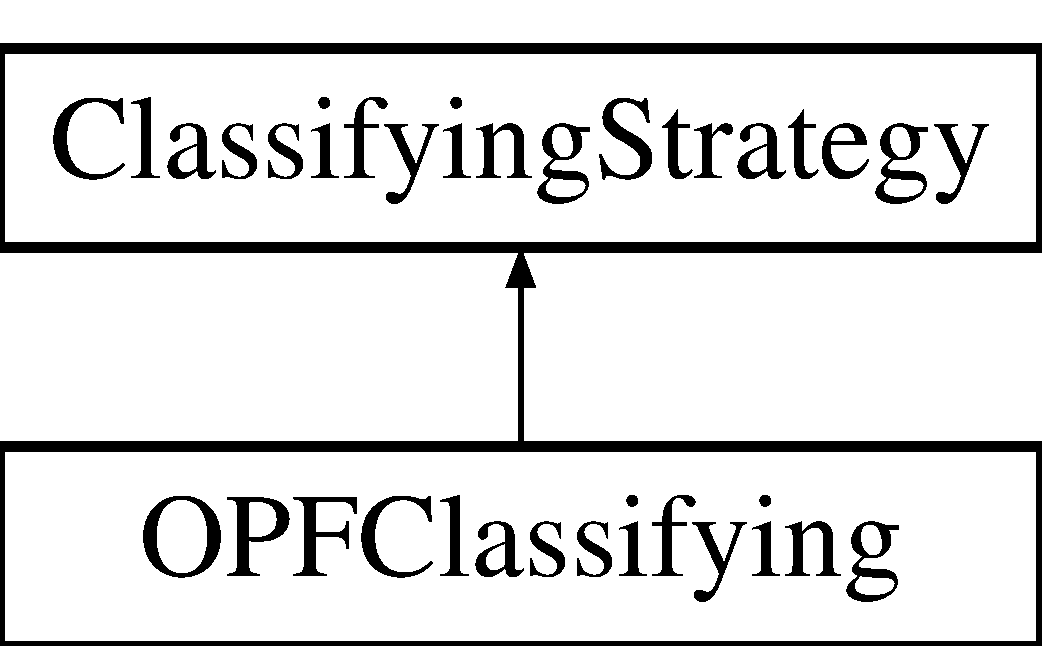
\includegraphics[height=2.000000cm]{classClassifyingStrategy}
\end{center}
\end{figure}
\subsection*{Public Member Functions}
\begin{DoxyCompactItemize}
\item 
\hyperlink{classClassifyingStrategy_a8dd920216306e6df413a9e5e0b34d93b}{Classifying\+Strategy} ()
\item 
virtual vector$<$ double $>$ \hyperlink{classClassifyingStrategy_a0b0e637921ba52ff52069824e96cab7b}{classify} (\hyperlink{classModel}{Model} model, \hyperlink{classPatterns}{Patterns} test)
\begin{DoxyCompactList}\small\item\em Returns a vector with predicted class values for all pattern in the set test. \end{DoxyCompactList}\end{DoxyCompactItemize}


\subsection{Detailed Description}
Interface for classifying strategies. 

One may want to develop a new \hyperlink{classOPF}{O\+P\+F} classifying strategy. Thus, this class provides an interface to support this development. All new classifying strategies should implement this interface. \begin{DoxyAuthor}{Authors}
Alan Zanoni Peixinho \href{mailto:apeixinho@studends.ic.unicamp.br}{\tt apeixinho@studends.\+ic.\+unicamp.\+br} 

Luis Augusto Martins Pereria \href{mailto:lmartins@ic.unicamb.br}{\tt lmartins@ic.\+unicamb.\+br} 
\end{DoxyAuthor}
\begin{DoxyVersion}{Version}
1.\+0.\+0 
\end{DoxyVersion}


\subsection{Constructor \& Destructor Documentation}
\hypertarget{classClassifyingStrategy_a8dd920216306e6df413a9e5e0b34d93b}{\index{Classifying\+Strategy@{Classifying\+Strategy}!Classifying\+Strategy@{Classifying\+Strategy}}
\index{Classifying\+Strategy@{Classifying\+Strategy}!Classifying\+Strategy@{Classifying\+Strategy}}
\subsubsection[{Classifying\+Strategy}]{\setlength{\rightskip}{0pt plus 5cm}Classifying\+Strategy\+::\+Classifying\+Strategy (
\begin{DoxyParamCaption}
{}
\end{DoxyParamCaption}
)}}\label{classClassifyingStrategy_a8dd920216306e6df413a9e5e0b34d93b}


\subsection{Member Function Documentation}
\hypertarget{classClassifyingStrategy_a0b0e637921ba52ff52069824e96cab7b}{\index{Classifying\+Strategy@{Classifying\+Strategy}!classify@{classify}}
\index{classify@{classify}!Classifying\+Strategy@{Classifying\+Strategy}}
\subsubsection[{classify}]{\setlength{\rightskip}{0pt plus 5cm}virtual vector$<$double$>$ Classifying\+Strategy\+::classify (
\begin{DoxyParamCaption}
\item[{{\bf Model}}]{model, }
\item[{{\bf Patterns}}]{test}
\end{DoxyParamCaption}
)\hspace{0.3cm}{\ttfamily [virtual]}}}\label{classClassifyingStrategy_a0b0e637921ba52ff52069824e96cab7b}


Returns a vector with predicted class values for all pattern in the set test. 

Predicted class values are placed into the vector following the same order of patterns in test set. 
\begin{DoxyParams}{Parameters}
{\em model} & a training model \\
\hline
\end{DoxyParams}
\begin{DoxyRefDesc}{Test}
\item[\hyperlink{test__test000001}{Test}]test set of patterns. \begin{DoxySeeAlso}{See Also}
\hyperlink{classOPFClassifying}{O\+P\+F\+Classifying} 
\end{DoxySeeAlso}
\end{DoxyRefDesc}


The documentation for this class was generated from the following file\+:\begin{DoxyCompactItemize}
\item 
Core/include/classifier/core/\hyperlink{classifying__strategy_8h}{classifying\+\_\+strategy.\+h}\end{DoxyCompactItemize}

\hypertarget{classCsvAdapter}{\section{Csv\+Adapter Class Reference}
\label{classCsvAdapter}\index{Csv\+Adapter@{Csv\+Adapter}}
}


{\ttfamily \#include $<$file\+\_\+formats.\+h$>$}

\subsection*{Public Member Functions}
\begin{DoxyCompactItemize}
\item 
\hyperlink{classCsvAdapter_a64b1bef0e0fdcba81f2c0d94b38ab0a0}{Csv\+Adapter} (\hyperlink{classPatterns}{Patterns} \&patterns)
\end{DoxyCompactItemize}
\subsection*{Friends}
\begin{DoxyCompactItemize}
\item 
istream \& \hyperlink{classCsvAdapter_a2a2e2f128a329757f385bbd6d0d3f0b4}{operator$>$$>$} (istream \&in, \hyperlink{classCsvAdapter}{Csv\+Adapter} \&c)
\end{DoxyCompactItemize}


\subsection{Constructor \& Destructor Documentation}
\hypertarget{classCsvAdapter_a64b1bef0e0fdcba81f2c0d94b38ab0a0}{\index{Csv\+Adapter@{Csv\+Adapter}!Csv\+Adapter@{Csv\+Adapter}}
\index{Csv\+Adapter@{Csv\+Adapter}!Csv\+Adapter@{Csv\+Adapter}}
\subsubsection[{Csv\+Adapter}]{\setlength{\rightskip}{0pt plus 5cm}Csv\+Adapter\+::\+Csv\+Adapter (
\begin{DoxyParamCaption}
\item[{{\bf Patterns} \&}]{patterns}
\end{DoxyParamCaption}
)}}\label{classCsvAdapter_a64b1bef0e0fdcba81f2c0d94b38ab0a0}


\subsection{Friends And Related Function Documentation}
\hypertarget{classCsvAdapter_a2a2e2f128a329757f385bbd6d0d3f0b4}{\index{Csv\+Adapter@{Csv\+Adapter}!operator$>$$>$@{operator$>$$>$}}
\index{operator$>$$>$@{operator$>$$>$}!Csv\+Adapter@{Csv\+Adapter}}
\subsubsection[{operator$>$$>$}]{\setlength{\rightskip}{0pt plus 5cm}istream\& operator$>$$>$ (
\begin{DoxyParamCaption}
\item[{istream \&}]{in, }
\item[{{\bf Csv\+Adapter} \&}]{c}
\end{DoxyParamCaption}
)\hspace{0.3cm}{\ttfamily [friend]}}}\label{classCsvAdapter_a2a2e2f128a329757f385bbd6d0d3f0b4}


The documentation for this class was generated from the following files\+:\begin{DoxyCompactItemize}
\item 
Core/include/input/\hyperlink{file__formats_8h}{file\+\_\+formats.\+h}\item 
Core/src/input/\hyperlink{file__formats_8cpp}{file\+\_\+formats.\+cpp}\end{DoxyCompactItemize}

\hypertarget{classMaxPolicy}{\section{Max\+Policy Class Reference}
\label{classMaxPolicy}\index{Max\+Policy@{Max\+Policy}}
}
\subsection*{Public Member Functions}
\begin{DoxyCompactItemize}
\item 
\hyperlink{classMaxPolicy_a69154bb395b6ab4c5e2cc51c29e68bed}{Max\+Policy} (int $\ast$index, double $\ast$cost)
\item 
bool \hyperlink{classMaxPolicy_a812f133c0ec9ce8d05fc7f53f4d001f9}{operator()} (int index1, int index2)
\end{DoxyCompactItemize}
\subsection*{Public Attributes}
\begin{DoxyCompactItemize}
\item 
int $\ast$ \hyperlink{classMaxPolicy_aa17f41977c819127778122aadc346660}{index\+\_\+}
\item 
double $\ast$ \hyperlink{classMaxPolicy_a043674b1b1737b2aaf7e29985693142a}{cost\+\_\+}
\end{DoxyCompactItemize}


\subsection{Constructor \& Destructor Documentation}
\hypertarget{classMaxPolicy_a69154bb395b6ab4c5e2cc51c29e68bed}{\index{Max\+Policy@{Max\+Policy}!Max\+Policy@{Max\+Policy}}
\index{Max\+Policy@{Max\+Policy}!Max\+Policy@{Max\+Policy}}
\subsubsection[{Max\+Policy}]{\setlength{\rightskip}{0pt plus 5cm}Max\+Policy\+::\+Max\+Policy (
\begin{DoxyParamCaption}
\item[{int $\ast$}]{index, }
\item[{double $\ast$}]{cost}
\end{DoxyParamCaption}
)\hspace{0.3cm}{\ttfamily [inline]}}}\label{classMaxPolicy_a69154bb395b6ab4c5e2cc51c29e68bed}


\subsection{Member Function Documentation}
\hypertarget{classMaxPolicy_a812f133c0ec9ce8d05fc7f53f4d001f9}{\index{Max\+Policy@{Max\+Policy}!operator()@{operator()}}
\index{operator()@{operator()}!Max\+Policy@{Max\+Policy}}
\subsubsection[{operator()}]{\setlength{\rightskip}{0pt plus 5cm}bool Max\+Policy\+::operator() (
\begin{DoxyParamCaption}
\item[{int}]{index1, }
\item[{int}]{index2}
\end{DoxyParamCaption}
)\hspace{0.3cm}{\ttfamily [inline]}}}\label{classMaxPolicy_a812f133c0ec9ce8d05fc7f53f4d001f9}


\subsection{Member Data Documentation}
\hypertarget{classMaxPolicy_a043674b1b1737b2aaf7e29985693142a}{\index{Max\+Policy@{Max\+Policy}!cost\+\_\+@{cost\+\_\+}}
\index{cost\+\_\+@{cost\+\_\+}!Max\+Policy@{Max\+Policy}}
\subsubsection[{cost\+\_\+}]{\setlength{\rightskip}{0pt plus 5cm}double$\ast$ Max\+Policy\+::cost\+\_\+}}\label{classMaxPolicy_a043674b1b1737b2aaf7e29985693142a}
\hypertarget{classMaxPolicy_aa17f41977c819127778122aadc346660}{\index{Max\+Policy@{Max\+Policy}!index\+\_\+@{index\+\_\+}}
\index{index\+\_\+@{index\+\_\+}!Max\+Policy@{Max\+Policy}}
\subsubsection[{index\+\_\+}]{\setlength{\rightskip}{0pt plus 5cm}int$\ast$ Max\+Policy\+::index\+\_\+}}\label{classMaxPolicy_aa17f41977c819127778122aadc346660}


The documentation for this class was generated from the following file\+:\begin{DoxyCompactItemize}
\item 
Core/src/utils/\hyperlink{priority__queue_8cpp}{priority\+\_\+queue.\+cpp}\end{DoxyCompactItemize}

\hypertarget{classMinPolicy}{\section{Min\+Policy Class Reference}
\label{classMinPolicy}\index{Min\+Policy@{Min\+Policy}}
}
\subsection*{Public Member Functions}
\begin{DoxyCompactItemize}
\item 
\hyperlink{classMinPolicy_ab16af4db33006558fc24b739b243f335}{Min\+Policy} (int $\ast$index, double $\ast$cost)
\item 
bool \hyperlink{classMinPolicy_a59891945c51d479ede8f7ed3def4b783}{operator()} (int index1, int index2)
\end{DoxyCompactItemize}
\subsection*{Public Attributes}
\begin{DoxyCompactItemize}
\item 
int $\ast$ \hyperlink{classMinPolicy_a45c577cd2a2fd0b6df22c0188a5a122c}{index\+\_\+}
\item 
double $\ast$ \hyperlink{classMinPolicy_abc47d408ac95a36297971f47513db31b}{cost\+\_\+}
\end{DoxyCompactItemize}


\subsection{Constructor \& Destructor Documentation}
\hypertarget{classMinPolicy_ab16af4db33006558fc24b739b243f335}{\index{Min\+Policy@{Min\+Policy}!Min\+Policy@{Min\+Policy}}
\index{Min\+Policy@{Min\+Policy}!Min\+Policy@{Min\+Policy}}
\subsubsection[{Min\+Policy}]{\setlength{\rightskip}{0pt plus 5cm}Min\+Policy\+::\+Min\+Policy (
\begin{DoxyParamCaption}
\item[{int $\ast$}]{index, }
\item[{double $\ast$}]{cost}
\end{DoxyParamCaption}
)\hspace{0.3cm}{\ttfamily [inline]}}}\label{classMinPolicy_ab16af4db33006558fc24b739b243f335}


\subsection{Member Function Documentation}
\hypertarget{classMinPolicy_a59891945c51d479ede8f7ed3def4b783}{\index{Min\+Policy@{Min\+Policy}!operator()@{operator()}}
\index{operator()@{operator()}!Min\+Policy@{Min\+Policy}}
\subsubsection[{operator()}]{\setlength{\rightskip}{0pt plus 5cm}bool Min\+Policy\+::operator() (
\begin{DoxyParamCaption}
\item[{int}]{index1, }
\item[{int}]{index2}
\end{DoxyParamCaption}
)\hspace{0.3cm}{\ttfamily [inline]}}}\label{classMinPolicy_a59891945c51d479ede8f7ed3def4b783}


\subsection{Member Data Documentation}
\hypertarget{classMinPolicy_abc47d408ac95a36297971f47513db31b}{\index{Min\+Policy@{Min\+Policy}!cost\+\_\+@{cost\+\_\+}}
\index{cost\+\_\+@{cost\+\_\+}!Min\+Policy@{Min\+Policy}}
\subsubsection[{cost\+\_\+}]{\setlength{\rightskip}{0pt plus 5cm}double$\ast$ Min\+Policy\+::cost\+\_\+}}\label{classMinPolicy_abc47d408ac95a36297971f47513db31b}
\hypertarget{classMinPolicy_a45c577cd2a2fd0b6df22c0188a5a122c}{\index{Min\+Policy@{Min\+Policy}!index\+\_\+@{index\+\_\+}}
\index{index\+\_\+@{index\+\_\+}!Min\+Policy@{Min\+Policy}}
\subsubsection[{index\+\_\+}]{\setlength{\rightskip}{0pt plus 5cm}int$\ast$ Min\+Policy\+::index\+\_\+}}\label{classMinPolicy_a45c577cd2a2fd0b6df22c0188a5a122c}


The documentation for this class was generated from the following file\+:\begin{DoxyCompactItemize}
\item 
Core/src/utils/\hyperlink{priority__queue_8cpp}{priority\+\_\+queue.\+cpp}\end{DoxyCompactItemize}

\hypertarget{classModel}{\section{Model Class Reference}
\label{classModel}\index{Model@{Model}}
}


Class for handling the training model informations.  




{\ttfamily \#include $<$model.\+h$>$}

\subsection*{Public Member Functions}
\begin{DoxyCompactItemize}
\item 
\hyperlink{classModel_a2970c96c9a3976c0887cb06f71753f1e}{Model} (\hyperlink{classPattern}{Pattern} pattern)
\item 
\hyperlink{classModel_a555e27949c7a209f607d77e5d57c1599}{Model} (string file\+\_\+name)
\begin{DoxyCompactList}\small\item\em Constructor for a model saved in file. \end{DoxyCompactList}\item 
vector$<$ int $>$ \hyperlink{classModel_ad821b67839a18f6fc6af508823ba73e0}{get\+\_\+ordered\+\_\+list\+\_\+of\+\_\+nodes} () const 
\item 
void \hyperlink{classModel_a6f2fa936b9d754d971f2972716b41656}{push\+\_\+ordered\+\_\+list\+\_\+of\+\_\+nodes} (int index)
\item 
Model\+Node $\ast$ \hyperlink{classModel_a7bae5e69e7ca1d5bb8a04c74148c82f0}{pop\+\_\+ordered\+\_\+list\+\_\+of\+\_\+nodes} () const 
\item 
vector$<$ Model\+Node $>$\+::\hyperlink{classModel_a0cfbe847990e80cb9033e8a3257bced2}{iterator} \hyperlink{classModel_a035c58a162aad06dad63a2be8976e17c}{begin} () const 
\item 
vector$<$ Model\+Node $>$\+::\hyperlink{classModel_a0cfbe847990e80cb9033e8a3257bced2}{iterator} \hyperlink{classModel_ad66f8045b3632a366af4f38b2042cf19}{end} () const 
\item 
std\+::ostream \& \hyperlink{classModel_a466e585afab385972eea3c8bd51f14f8}{operator$>$$>$} (std\+::ostream \&out)
\item 
void \hyperlink{classModel_afa9087f16c68b0c7cb67c5a285dde750}{save\+\_\+model\+\_\+to\+\_\+file} ()
\begin{DoxyCompactList}\small\item\em Save model to file. \end{DoxyCompactList}\end{DoxyCompactItemize}
\subsection*{Public Attributes}
\begin{DoxyCompactItemize}
\item 
vector$<$ Model\+Node $>$\+::iterator \hyperlink{classModel_a0cfbe847990e80cb9033e8a3257bced2}{iterator}
\item 
vector$<$ Model\+Node $>$\+::const\+\_\+iterator \hyperlink{classModel_a578f203623cdda48b577f10a8d6e12d4}{const\+\_\+iterator}
\end{DoxyCompactItemize}
\subsection*{Private Member Functions}
\begin{DoxyCompactItemize}
\item 
void \hyperlink{classModel_a020fe8b33fb2c430fe42a95e1ea83df4}{load\+\_\+model\+\_\+from\+\_\+file} (string file\+\_\+name)
\begin{DoxyCompactList}\small\item\em Loads a model from file. \end{DoxyCompactList}\end{DoxyCompactItemize}
\subsection*{Private Attributes}
\begin{DoxyCompactItemize}
\item 
vector$<$ int $>$ \hyperlink{classModel_a3324528ad5418b5d1a1a9a4b2a24e6e8}{ordered\+\_\+list\+\_\+of\+\_\+nodes\+\_\+}
\item 
vector$<$ Model\+Node $>$ \hyperlink{classModel_abf34f73f474d2eb05d2aa285cb88b828}{node}
\end{DoxyCompactItemize}


\subsection{Detailed Description}
Class for handling the training model informations. 

This class provides attributes and methods to deal with information arising from training process that will be used on classifying process. Among the informations that model can handle are\+: cost paths, set of pattern using in training phase, learned class value, predecessor of a node and so on. \begin{DoxyAuthor}{Authors}
Alan Zanoni Peixinho \href{mailto:apeixinho@studends.ic.unicamp.br}{\tt apeixinho@studends.\+ic.\+unicamp.\+br} 

Luis Augusto Martins Pereria \href{mailto:lmartins@ic.unicamb.br}{\tt lmartins@ic.\+unicamb.\+br} 
\end{DoxyAuthor}
\begin{DoxyVersion}{Version}
1.\+0.\+0 
\end{DoxyVersion}


\subsection{Constructor \& Destructor Documentation}
\hypertarget{classModel_a2970c96c9a3976c0887cb06f71753f1e}{\index{Model@{Model}!Model@{Model}}
\index{Model@{Model}!Model@{Model}}
\subsubsection[{Model}]{\setlength{\rightskip}{0pt plus 5cm}Model\+::\+Model (
\begin{DoxyParamCaption}
\item[{{\bf Pattern}}]{pattern}
\end{DoxyParamCaption}
)}}\label{classModel_a2970c96c9a3976c0887cb06f71753f1e}
\hypertarget{classModel_a555e27949c7a209f607d77e5d57c1599}{\index{Model@{Model}!Model@{Model}}
\index{Model@{Model}!Model@{Model}}
\subsubsection[{Model}]{\setlength{\rightskip}{0pt plus 5cm}Model\+::\+Model (
\begin{DoxyParamCaption}
\item[{string}]{file\+\_\+name}
\end{DoxyParamCaption}
)}}\label{classModel_a555e27949c7a209f607d77e5d57c1599}


Constructor for a model saved in file. 


\begin{DoxyParams}{Parameters}
{\em file\+\_\+name} & name of a file whose model was saved in. \\
\hline
\end{DoxyParams}


\subsection{Member Function Documentation}
\hypertarget{classModel_a035c58a162aad06dad63a2be8976e17c}{\index{Model@{Model}!begin@{begin}}
\index{begin@{begin}!Model@{Model}}
\subsubsection[{begin}]{\setlength{\rightskip}{0pt plus 5cm}{\bf iterator} Model\+::begin (
\begin{DoxyParamCaption}
{}
\end{DoxyParamCaption}
) const}}\label{classModel_a035c58a162aad06dad63a2be8976e17c}
\hypertarget{classModel_ad66f8045b3632a366af4f38b2042cf19}{\index{Model@{Model}!end@{end}}
\index{end@{end}!Model@{Model}}
\subsubsection[{end}]{\setlength{\rightskip}{0pt plus 5cm}{\bf iterator} Model\+::end (
\begin{DoxyParamCaption}
{}
\end{DoxyParamCaption}
) const}}\label{classModel_ad66f8045b3632a366af4f38b2042cf19}
\hypertarget{classModel_ad821b67839a18f6fc6af508823ba73e0}{\index{Model@{Model}!get\+\_\+ordered\+\_\+list\+\_\+of\+\_\+nodes@{get\+\_\+ordered\+\_\+list\+\_\+of\+\_\+nodes}}
\index{get\+\_\+ordered\+\_\+list\+\_\+of\+\_\+nodes@{get\+\_\+ordered\+\_\+list\+\_\+of\+\_\+nodes}!Model@{Model}}
\subsubsection[{get\+\_\+ordered\+\_\+list\+\_\+of\+\_\+nodes}]{\setlength{\rightskip}{0pt plus 5cm}vector$<$ int $>$ Model\+::get\+\_\+ordered\+\_\+list\+\_\+of\+\_\+nodes (
\begin{DoxyParamCaption}
{}
\end{DoxyParamCaption}
) const\hspace{0.3cm}{\ttfamily [inline]}}}\label{classModel_ad821b67839a18f6fc6af508823ba73e0}
\hypertarget{classModel_a020fe8b33fb2c430fe42a95e1ea83df4}{\index{Model@{Model}!load\+\_\+model\+\_\+from\+\_\+file@{load\+\_\+model\+\_\+from\+\_\+file}}
\index{load\+\_\+model\+\_\+from\+\_\+file@{load\+\_\+model\+\_\+from\+\_\+file}!Model@{Model}}
\subsubsection[{load\+\_\+model\+\_\+from\+\_\+file}]{\setlength{\rightskip}{0pt plus 5cm}void Model\+::load\+\_\+model\+\_\+from\+\_\+file (
\begin{DoxyParamCaption}
\item[{string}]{file\+\_\+name}
\end{DoxyParamCaption}
)\hspace{0.3cm}{\ttfamily [private]}}}\label{classModel_a020fe8b33fb2c430fe42a95e1ea83df4}


Loads a model from file. 

File has to be saved using save\+\_\+model\+\_\+to\+\_\+file. \begin{DoxySeeAlso}{See Also}
\hyperlink{classModel_afa9087f16c68b0c7cb67c5a285dde750}{save\+\_\+model\+\_\+to\+\_\+file} 
\end{DoxySeeAlso}
\hypertarget{classModel_a466e585afab385972eea3c8bd51f14f8}{\index{Model@{Model}!operator$>$$>$@{operator$>$$>$}}
\index{operator$>$$>$@{operator$>$$>$}!Model@{Model}}
\subsubsection[{operator$>$$>$}]{\setlength{\rightskip}{0pt plus 5cm}std\+::ostream\& Model\+::operator$>$$>$ (
\begin{DoxyParamCaption}
\item[{std\+::ostream \&}]{out}
\end{DoxyParamCaption}
)}}\label{classModel_a466e585afab385972eea3c8bd51f14f8}
\hypertarget{classModel_a7bae5e69e7ca1d5bb8a04c74148c82f0}{\index{Model@{Model}!pop\+\_\+ordered\+\_\+list\+\_\+of\+\_\+nodes@{pop\+\_\+ordered\+\_\+list\+\_\+of\+\_\+nodes}}
\index{pop\+\_\+ordered\+\_\+list\+\_\+of\+\_\+nodes@{pop\+\_\+ordered\+\_\+list\+\_\+of\+\_\+nodes}!Model@{Model}}
\subsubsection[{pop\+\_\+ordered\+\_\+list\+\_\+of\+\_\+nodes}]{\setlength{\rightskip}{0pt plus 5cm}Model\+Node $\ast$ Model\+::pop\+\_\+ordered\+\_\+list\+\_\+of\+\_\+nodes (
\begin{DoxyParamCaption}
{}
\end{DoxyParamCaption}
) const}}\label{classModel_a7bae5e69e7ca1d5bb8a04c74148c82f0}
\hypertarget{classModel_a6f2fa936b9d754d971f2972716b41656}{\index{Model@{Model}!push\+\_\+ordered\+\_\+list\+\_\+of\+\_\+nodes@{push\+\_\+ordered\+\_\+list\+\_\+of\+\_\+nodes}}
\index{push\+\_\+ordered\+\_\+list\+\_\+of\+\_\+nodes@{push\+\_\+ordered\+\_\+list\+\_\+of\+\_\+nodes}!Model@{Model}}
\subsubsection[{push\+\_\+ordered\+\_\+list\+\_\+of\+\_\+nodes}]{\setlength{\rightskip}{0pt plus 5cm}void Model\+::push\+\_\+ordered\+\_\+list\+\_\+of\+\_\+nodes (
\begin{DoxyParamCaption}
\item[{int}]{index}
\end{DoxyParamCaption}
)}}\label{classModel_a6f2fa936b9d754d971f2972716b41656}
\hypertarget{classModel_afa9087f16c68b0c7cb67c5a285dde750}{\index{Model@{Model}!save\+\_\+model\+\_\+to\+\_\+file@{save\+\_\+model\+\_\+to\+\_\+file}}
\index{save\+\_\+model\+\_\+to\+\_\+file@{save\+\_\+model\+\_\+to\+\_\+file}!Model@{Model}}
\subsubsection[{save\+\_\+model\+\_\+to\+\_\+file}]{\setlength{\rightskip}{0pt plus 5cm}void Model\+::save\+\_\+model\+\_\+to\+\_\+file (
\begin{DoxyParamCaption}
{}
\end{DoxyParamCaption}
)}}\label{classModel_afa9087f16c68b0c7cb67c5a285dde750}


Save model to file. 

\hyperlink{classModel}{Model} has to be completely filled. 

\subsection{Member Data Documentation}
\hypertarget{classModel_a578f203623cdda48b577f10a8d6e12d4}{\index{Model@{Model}!const\+\_\+iterator@{const\+\_\+iterator}}
\index{const\+\_\+iterator@{const\+\_\+iterator}!Model@{Model}}
\subsubsection[{const\+\_\+iterator}]{\setlength{\rightskip}{0pt plus 5cm}vector$<$Model\+Node$>$\+::const\+\_\+iterator Model\+::const\+\_\+iterator}}\label{classModel_a578f203623cdda48b577f10a8d6e12d4}
\hypertarget{classModel_a0cfbe847990e80cb9033e8a3257bced2}{\index{Model@{Model}!iterator@{iterator}}
\index{iterator@{iterator}!Model@{Model}}
\subsubsection[{iterator}]{\setlength{\rightskip}{0pt plus 5cm}vector$<$Model\+Node$>$\+::iterator Model\+::iterator}}\label{classModel_a0cfbe847990e80cb9033e8a3257bced2}
\hypertarget{classModel_abf34f73f474d2eb05d2aa285cb88b828}{\index{Model@{Model}!node@{node}}
\index{node@{node}!Model@{Model}}
\subsubsection[{node}]{\setlength{\rightskip}{0pt plus 5cm}vector$<$Model\+Node$>$ Model\+::node\hspace{0.3cm}{\ttfamily [private]}}}\label{classModel_abf34f73f474d2eb05d2aa285cb88b828}
\hypertarget{classModel_a3324528ad5418b5d1a1a9a4b2a24e6e8}{\index{Model@{Model}!ordered\+\_\+list\+\_\+of\+\_\+nodes\+\_\+@{ordered\+\_\+list\+\_\+of\+\_\+nodes\+\_\+}}
\index{ordered\+\_\+list\+\_\+of\+\_\+nodes\+\_\+@{ordered\+\_\+list\+\_\+of\+\_\+nodes\+\_\+}!Model@{Model}}
\subsubsection[{ordered\+\_\+list\+\_\+of\+\_\+nodes\+\_\+}]{\setlength{\rightskip}{0pt plus 5cm}vector$<$int$>$ Model\+::ordered\+\_\+list\+\_\+of\+\_\+nodes\+\_\+\hspace{0.3cm}{\ttfamily [private]}}}\label{classModel_a3324528ad5418b5d1a1a9a4b2a24e6e8}


The documentation for this class was generated from the following files\+:\begin{DoxyCompactItemize}
\item 
Core/include/classifier/core/\hyperlink{model_8h}{model.\+h}\item 
Core/src/classifier/core/\hyperlink{model_8cpp}{model.\+cpp}\end{DoxyCompactItemize}

\hypertarget{classMSTPrototypes}{\section{M\+S\+T\+Prototypes Class Reference}
\label{classMSTPrototypes}\index{M\+S\+T\+Prototypes@{M\+S\+T\+Prototypes}}
}


Class to handle prototypes selection by using a Minimum Spanning Tree (M\+S\+T).  




{\ttfamily \#include $<$mst\+\_\+prototype.\+h$>$}

Inheritance diagram for M\+S\+T\+Prototypes\+:\begin{figure}[H]
\begin{center}
\leavevmode
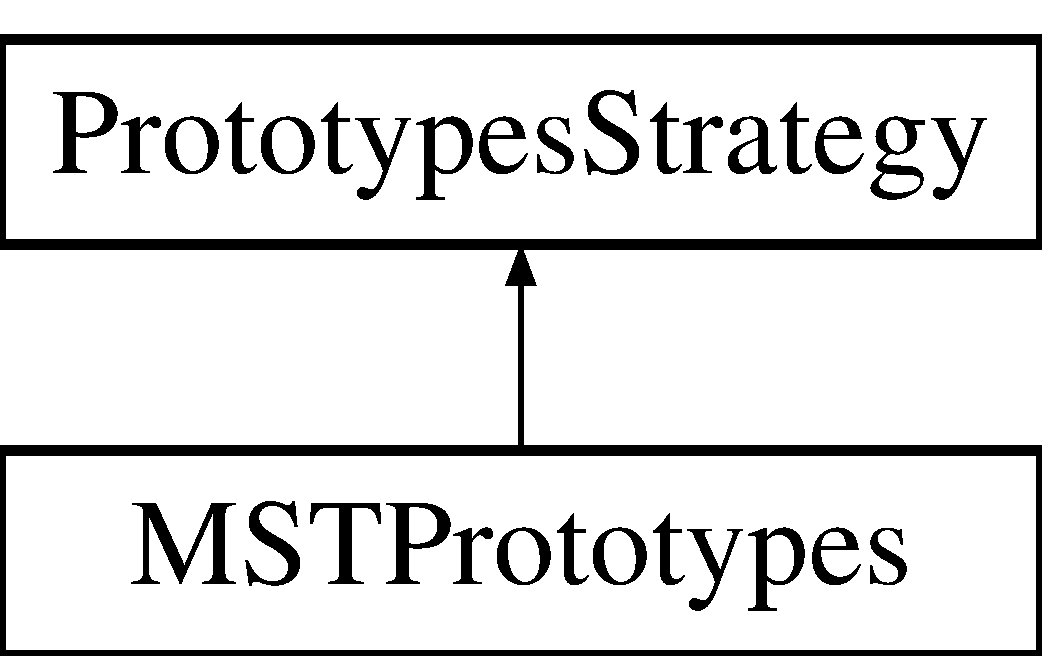
\includegraphics[height=2.000000cm]{classMSTPrototypes}
\end{center}
\end{figure}
\subsection*{Public Member Functions}
\begin{DoxyCompactItemize}
\item 
\hyperlink{classMSTPrototypes_a62fedec88ad4ab417181fbc672f72410}{M\+S\+T\+Prototypes} ()
\item 
virtual vector$<$ double $>$ \hyperlink{classMSTPrototypes_a654ccbaebfdbca73a0da0e5eb1e4e39f}{Select\+Prototypes} (\hyperlink{namespaceopf_a61631393754e0aa6aaeacf0767b2b419}{opf\+::\+Distance} distance, \hyperlink{classPatterns}{Patterns} patterns)
\begin{DoxyCompactList}\small\item\em Returns a array of size of patterns with zero value is a pattern is a prototype and infinity otherwise. \end{DoxyCompactList}\end{DoxyCompactItemize}


\subsection{Detailed Description}
Class to handle prototypes selection by using a Minimum Spanning Tree (M\+S\+T). 

Prim's algorithm is performed to generate the M\+S\+T. Two patterns on M\+S\+T are selected as prototypes if they are connected and belong to different classes. 

\subsection{Constructor \& Destructor Documentation}
\hypertarget{classMSTPrototypes_a62fedec88ad4ab417181fbc672f72410}{\index{M\+S\+T\+Prototypes@{M\+S\+T\+Prototypes}!M\+S\+T\+Prototypes@{M\+S\+T\+Prototypes}}
\index{M\+S\+T\+Prototypes@{M\+S\+T\+Prototypes}!M\+S\+T\+Prototypes@{M\+S\+T\+Prototypes}}
\subsubsection[{M\+S\+T\+Prototypes}]{\setlength{\rightskip}{0pt plus 5cm}M\+S\+T\+Prototypes\+::\+M\+S\+T\+Prototypes (
\begin{DoxyParamCaption}
{}
\end{DoxyParamCaption}
)}}\label{classMSTPrototypes_a62fedec88ad4ab417181fbc672f72410}


\subsection{Member Function Documentation}
\hypertarget{classMSTPrototypes_a654ccbaebfdbca73a0da0e5eb1e4e39f}{\index{M\+S\+T\+Prototypes@{M\+S\+T\+Prototypes}!Select\+Prototypes@{Select\+Prototypes}}
\index{Select\+Prototypes@{Select\+Prototypes}!M\+S\+T\+Prototypes@{M\+S\+T\+Prototypes}}
\subsubsection[{Select\+Prototypes}]{\setlength{\rightskip}{0pt plus 5cm}vector$<$ double $>$ M\+S\+T\+Prototypes\+::\+Select\+Prototypes (
\begin{DoxyParamCaption}
\item[{{\bf opf\+::\+Distance}}]{distance, }
\item[{{\bf Patterns}}]{patterns}
\end{DoxyParamCaption}
)\hspace{0.3cm}{\ttfamily [virtual]}}}\label{classMSTPrototypes_a654ccbaebfdbca73a0da0e5eb1e4e39f}


Returns a array of size of patterns with zero value is a pattern is a prototype and infinity otherwise. 


\begin{DoxyParams}{Parameters}
{\em distance} & a distance function. \\
\hline
{\em patterns} & a set of single pattern. \\
\hline
\end{DoxyParams}


Implements \hyperlink{classPrototypesStrategy_a0422be14bb6be39a2d06112daf7043c1}{Prototypes\+Strategy}.



The documentation for this class was generated from the following files\+:\begin{DoxyCompactItemize}
\item 
Core/include/classifier/complete\+\_\+graph/\hyperlink{mst__prototype_8h}{mst\+\_\+prototype.\+h}\item 
Core/src/classifier/complete\+\_\+graph/\hyperlink{mst__prototype_8cpp}{mst\+\_\+prototype.\+cpp}\end{DoxyCompactItemize}

\hypertarget{classOPF}{\section{O\+P\+F Class Reference}
\label{classOPF}\index{O\+P\+F@{O\+P\+F}}
}


{\ttfamily \#include $<$opf.\+h$>$}

\subsection*{Public Member Functions}
\begin{DoxyCompactItemize}
\item 
\hyperlink{classOPF_a937d755f9ec9d517eead90e06d5ab672}{O\+P\+F} (\hyperlink{classTrainer}{Trainer} \&trainer, \hyperlink{classClassifier}{Classifier} \&classifier, \hyperlink{namespaceopf_a61631393754e0aa6aaeacf0767b2b419}{opf\+::\+Distance} distance)
\item 
void \hyperlink{classOPF_a3008876cfbc3879986126308ca23cc1e}{Build\+Model} (\hyperlink{classPatterns}{Patterns} \&training)
\item 
int \hyperlink{classOPF_a694477ddd6df7bebbd1856cdf7bf3ce1}{Predict} (\hyperlink{classPatterns}{Patterns} \&test)
\end{DoxyCompactItemize}
\subsection*{Private Attributes}
\begin{DoxyCompactItemize}
\item 
\hyperlink{classModel}{Model} $\ast$ \hyperlink{classOPF_a906ed713cbe0d20ffb96d064f4db42c1}{opf\+\_\+model\+\_\+} = N\+U\+L\+L
\end{DoxyCompactItemize}


\subsection{Detailed Description}
\begin{DoxyAuthor}{Authors}
Alan Zanoni Peixinho \href{mailto:apeixinho@studends.ic.unicamp.br}{\tt apeixinho@studends.\+ic.\+unicamp.\+br} 

Luis Augusto Martins Pereria \href{mailto:lmartins@ic.unicamb.br}{\tt lmartins@ic.\+unicamb.\+br} 
\end{DoxyAuthor}
\begin{DoxyVersion}{Version}
1.\+0.\+0 
\end{DoxyVersion}


\subsection{Constructor \& Destructor Documentation}
\hypertarget{classOPF_a937d755f9ec9d517eead90e06d5ab672}{\index{O\+P\+F@{O\+P\+F}!O\+P\+F@{O\+P\+F}}
\index{O\+P\+F@{O\+P\+F}!O\+P\+F@{O\+P\+F}}
\subsubsection[{O\+P\+F}]{\setlength{\rightskip}{0pt plus 5cm}O\+P\+F\+::\+O\+P\+F (
\begin{DoxyParamCaption}
\item[{{\bf Trainer} \&}]{trainer, }
\item[{{\bf Classifier} \&}]{classifier, }
\item[{{\bf opf\+::\+Distance}}]{distance}
\end{DoxyParamCaption}
)}}\label{classOPF_a937d755f9ec9d517eead90e06d5ab672}


\subsection{Member Function Documentation}
\hypertarget{classOPF_a3008876cfbc3879986126308ca23cc1e}{\index{O\+P\+F@{O\+P\+F}!Build\+Model@{Build\+Model}}
\index{Build\+Model@{Build\+Model}!O\+P\+F@{O\+P\+F}}
\subsubsection[{Build\+Model}]{\setlength{\rightskip}{0pt plus 5cm}void O\+P\+F\+::\+Build\+Model (
\begin{DoxyParamCaption}
\item[{{\bf Patterns} \&}]{training}
\end{DoxyParamCaption}
)}}\label{classOPF_a3008876cfbc3879986126308ca23cc1e}
\hypertarget{classOPF_a694477ddd6df7bebbd1856cdf7bf3ce1}{\index{O\+P\+F@{O\+P\+F}!Predict@{Predict}}
\index{Predict@{Predict}!O\+P\+F@{O\+P\+F}}
\subsubsection[{Predict}]{\setlength{\rightskip}{0pt plus 5cm}int O\+P\+F\+::\+Predict (
\begin{DoxyParamCaption}
\item[{{\bf Patterns} \&}]{test}
\end{DoxyParamCaption}
)}}\label{classOPF_a694477ddd6df7bebbd1856cdf7bf3ce1}


\subsection{Member Data Documentation}
\hypertarget{classOPF_a906ed713cbe0d20ffb96d064f4db42c1}{\index{O\+P\+F@{O\+P\+F}!opf\+\_\+model\+\_\+@{opf\+\_\+model\+\_\+}}
\index{opf\+\_\+model\+\_\+@{opf\+\_\+model\+\_\+}!O\+P\+F@{O\+P\+F}}
\subsubsection[{opf\+\_\+model\+\_\+}]{\setlength{\rightskip}{0pt plus 5cm}{\bf Model}$\ast$ O\+P\+F\+::opf\+\_\+model\+\_\+ = N\+U\+L\+L\hspace{0.3cm}{\ttfamily [private]}}}\label{classOPF_a906ed713cbe0d20ffb96d064f4db42c1}


The documentation for this class was generated from the following files\+:\begin{DoxyCompactItemize}
\item 
Core/include/classifier/core/\hyperlink{opf_8h}{opf.\+h}\item 
Core/src/classifier/core/\hyperlink{opf_8cpp}{opf.\+cpp}\end{DoxyCompactItemize}

\hypertarget{classOPFClassifying}{\section{O\+P\+F\+Classifying Class Reference}
\label{classOPFClassifying}\index{O\+P\+F\+Classifying@{O\+P\+F\+Classifying}}
}


Class to handle prototypes selection by using a Minimum Spanning Tree (M\+S\+T).  




{\ttfamily \#include $<$opf\+\_\+classifying.\+h$>$}

Inheritance diagram for O\+P\+F\+Classifying\+:\begin{figure}[H]
\begin{center}
\leavevmode
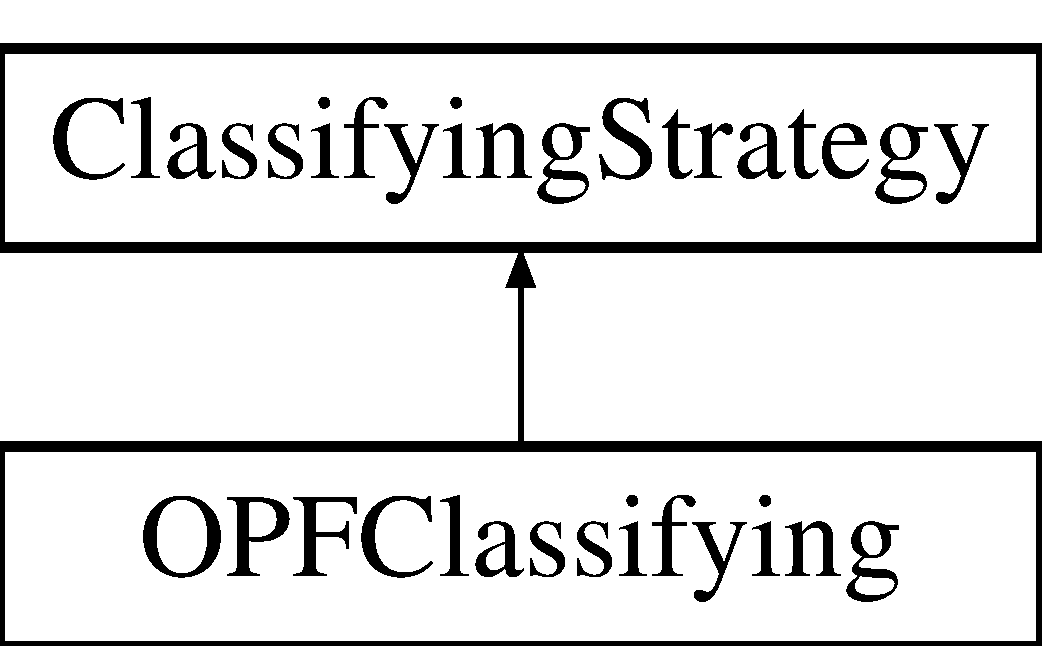
\includegraphics[height=2.000000cm]{classOPFClassifying}
\end{center}
\end{figure}
\subsection*{Additional Inherited Members}


\subsection{Detailed Description}
Class to handle prototypes selection by using a Minimum Spanning Tree (M\+S\+T). 

Prim's algorithm is performed to generate the M\+S\+T. Two patterns on M\+S\+T are selected as prototypes if they are connected and belong to different classes.

\begin{DoxyAuthor}{Authors}
Alan Zanoni Peixinho \href{mailto:apeixinho@studends.ic.unicamp.br}{\tt apeixinho@studends.\+ic.\+unicamp.\+br} 

Luis Augusto Martins Pereria \href{mailto:lmartins@ic.unicamb.br}{\tt lmartins@ic.\+unicamb.\+br} 
\end{DoxyAuthor}
\begin{DoxyVersion}{Version}
1.\+0.\+0 
\end{DoxyVersion}


The documentation for this class was generated from the following files\+:\begin{DoxyCompactItemize}
\item 
Core/include/classifier/complete\+\_\+graph/\hyperlink{opf__classifying_8h}{opf\+\_\+classifying.\+h}\item 
Core/src/classifier/complete\+\_\+graph/\hyperlink{opf__classifying_8cpp}{opf\+\_\+classifying.\+cpp}\end{DoxyCompactItemize}

\hypertarget{classOPFTraining}{\section{O\+P\+F\+Training Class Reference}
\label{classOPFTraining}\index{O\+P\+F\+Training@{O\+P\+F\+Training}}
}


{\ttfamily \#include $<$opf\+\_\+training.\+h$>$}

Inheritance diagram for O\+P\+F\+Training\+:\begin{figure}[H]
\begin{center}
\leavevmode
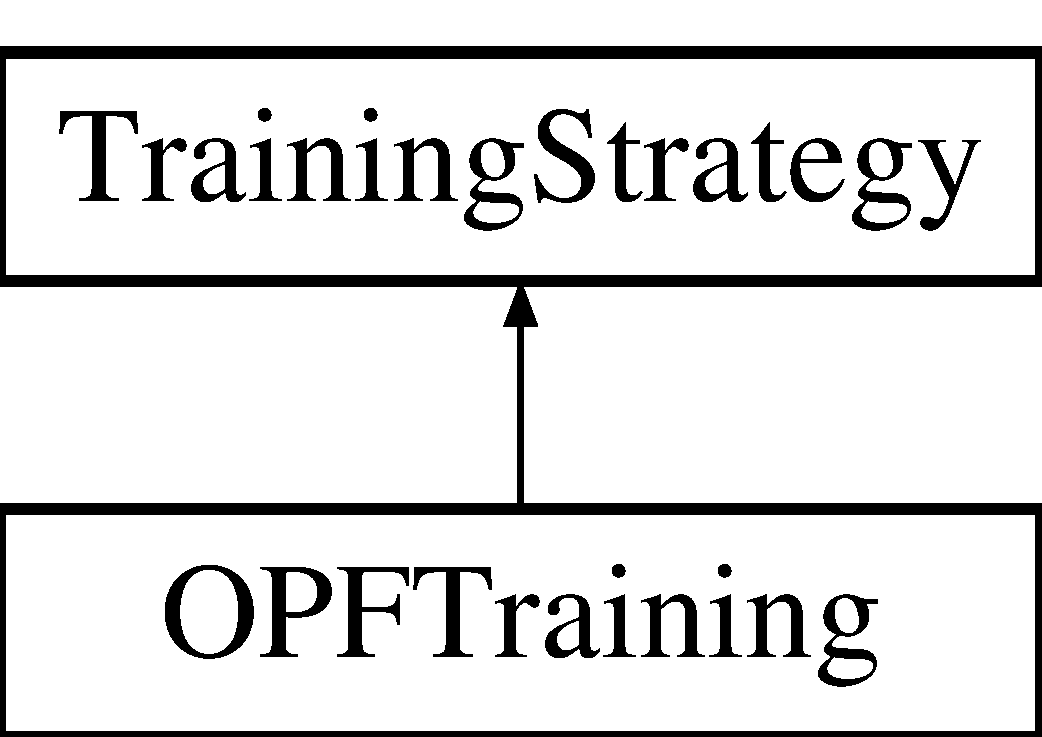
\includegraphics[height=2.000000cm]{classOPFTraining}
\end{center}
\end{figure}
\subsection*{Public Member Functions}
\begin{DoxyCompactItemize}
\item 
\hyperlink{classOPFTraining_a901f7f1c7f467dcfee5678fc4b6bfbd4}{O\+P\+F\+Training} ()
\item 
virtual \hyperlink{classModel}{Model} $\ast$ \hyperlink{classOPFTraining_a7ccc8643c9f973f7323cd6622b0bf616}{train} (\hyperlink{namespaceopf_a61631393754e0aa6aaeacf0767b2b419}{opf\+::\+Distance} distance, \hyperlink{classPatterns}{Patterns} patterns)
\item 
virtual \hyperlink{classModel}{Model} $\ast$ \hyperlink{classTrainingStrategy_ad5da56b8b57e010c97a782d9e629e2b5}{train} ()
\end{DoxyCompactItemize}


\subsection{Detailed Description}
\begin{DoxyAuthor}{Authors}
Alan Zanoni Peixinho \href{mailto:apeixinho@studends.ic.unicamp.br}{\tt apeixinho@studends.\+ic.\+unicamp.\+br} 

Luis Augusto Martins Pereria \href{mailto:lmartins@ic.unicamb.br}{\tt lmartins@ic.\+unicamb.\+br} 
\end{DoxyAuthor}
\begin{DoxyVersion}{Version}
1.\+0.\+0 
\end{DoxyVersion}


\subsection{Constructor \& Destructor Documentation}
\hypertarget{classOPFTraining_a901f7f1c7f467dcfee5678fc4b6bfbd4}{\index{O\+P\+F\+Training@{O\+P\+F\+Training}!O\+P\+F\+Training@{O\+P\+F\+Training}}
\index{O\+P\+F\+Training@{O\+P\+F\+Training}!O\+P\+F\+Training@{O\+P\+F\+Training}}
\subsubsection[{O\+P\+F\+Training}]{\setlength{\rightskip}{0pt plus 5cm}O\+P\+F\+Training\+::\+O\+P\+F\+Training (
\begin{DoxyParamCaption}
{}
\end{DoxyParamCaption}
)}}\label{classOPFTraining_a901f7f1c7f467dcfee5678fc4b6bfbd4}


\subsection{Member Function Documentation}
\hypertarget{classTrainingStrategy_ad5da56b8b57e010c97a782d9e629e2b5}{\index{O\+P\+F\+Training@{O\+P\+F\+Training}!train@{train}}
\index{train@{train}!O\+P\+F\+Training@{O\+P\+F\+Training}}
\subsubsection[{train}]{\setlength{\rightskip}{0pt plus 5cm}virtual {\bf Model}$\ast$ Training\+Strategy\+::train (
\begin{DoxyParamCaption}
{}
\end{DoxyParamCaption}
)\hspace{0.3cm}{\ttfamily [virtual]}, {\ttfamily [inherited]}}}\label{classTrainingStrategy_ad5da56b8b57e010c97a782d9e629e2b5}
\hypertarget{classOPFTraining_a7ccc8643c9f973f7323cd6622b0bf616}{\index{O\+P\+F\+Training@{O\+P\+F\+Training}!train@{train}}
\index{train@{train}!O\+P\+F\+Training@{O\+P\+F\+Training}}
\subsubsection[{train}]{\setlength{\rightskip}{0pt plus 5cm}{\bf Model} $\ast$ O\+P\+F\+Training\+::train (
\begin{DoxyParamCaption}
\item[{{\bf opf\+::\+Distance}}]{distance, }
\item[{{\bf Patterns}}]{patterns}
\end{DoxyParamCaption}
)\hspace{0.3cm}{\ttfamily [virtual]}}}\label{classOPFTraining_a7ccc8643c9f973f7323cd6622b0bf616}


The documentation for this class was generated from the following files\+:\begin{DoxyCompactItemize}
\item 
Core/include/classifier/complete\+\_\+graph/\hyperlink{opf__training_8h}{opf\+\_\+training.\+h}\item 
Core/src/classifier/complete\+\_\+graph/\hyperlink{opf__training_8cpp}{opf\+\_\+training.\+cpp}\end{DoxyCompactItemize}

\hypertarget{classPattern}{\section{Pattern Class Reference}
\label{classPattern}\index{Pattern@{Pattern}}
}


Class for handling a single pattern.  




{\ttfamily \#include $<$pattern.\+h$>$}

\subsection*{Public Member Functions}
\begin{DoxyCompactItemize}
\item 
\hyperlink{classPattern_a95f42b0f1717d9e6c2d831e87d27f83c}{Pattern} ()
\begin{DoxyCompactList}\small\item\em Standard constructor for a single pattern. \end{DoxyCompactList}\item 
{\footnotesize template$<$typename Iterator $>$ }\\\hyperlink{classPattern_a3cf22799a811394bab7fd167727a16af}{Pattern} (int class\+\_\+value, Iterator begin, Iterator end, int index)
\begin{DoxyCompactList}\small\item\em Constructor creating a labeled pattern. \end{DoxyCompactList}\item 
{\footnotesize template$<$typename Iterator $>$ }\\\hyperlink{classPattern_a87dcb126d751b5520a710dbf3e4eb7c0}{Pattern} (Iterator begin, Iterator end, int index)
\begin{DoxyCompactList}\small\item\em Constructor creating a unlabeled pattern. \end{DoxyCompactList}\item 
\hyperlink{classPattern_a3a1bf7ddd196fac02018c9cde4c421cf}{Pattern} (int dimension)
\begin{DoxyCompactList}\small\item\em Constructor creating a pattern allocating space to feature vector. \end{DoxyCompactList}\item 
\hyperlink{classPattern_a6e8b9388bbd39934e9f9534b974d7498}{$\sim$\+Pattern} ()
\begin{DoxyCompactList}\small\item\em Destructor for single pattern. \end{DoxyCompactList}\item 
int \hyperlink{classPattern_aae331219e63c782b23f203ebad3aa7bc}{get\+\_\+class\+\_\+value} () const 
\begin{DoxyCompactList}\small\item\em Returns the class value of the pattern. \end{DoxyCompactList}\item 
void \hyperlink{classPattern_ac4235d677a656d5cc272d192af210d4f}{set\+\_\+class\+\_\+value} (int class\+\_\+value)
\begin{DoxyCompactList}\small\item\em Sets the class value of the pattern. \end{DoxyCompactList}\item 
const vector$<$ double $>$ \hyperlink{classPattern_aae9583bcb7da91e9ae347a392ae77a52}{get\+\_\+feature\+\_\+vector} () const 
\begin{DoxyCompactList}\small\item\em Returns the feature vector of the pattern. \end{DoxyCompactList}\item 
{\footnotesize template$<$typename Iterator $>$ }\\void \hyperlink{classPattern_a325cfe99a75f6e2befccef37ea347135}{set\+\_\+feature\+\_\+vector} (Iterator begin, Iterator end)
\begin{DoxyCompactList}\small\item\em Sets the feature vector of the pattern. \end{DoxyCompactList}\item 
int \hyperlink{classPattern_a3301651f9617962a7dd15575d381d8de}{get\+\_\+dimension} () const 
\begin{DoxyCompactList}\small\item\em Returns the dimension size of feature vector. \end{DoxyCompactList}\item 
void \hyperlink{classPattern_aa498151def7e9e9fabf874bfead90b3b}{set\+\_\+dimension} (int dimension)
\begin{DoxyCompactList}\small\item\em Sets the dimension size of feature vector. \end{DoxyCompactList}\item 
int \hyperlink{classPattern_a96c0f3b51801a27d0f8b06031b508b42}{get\+\_\+index} () const 
\begin{DoxyCompactList}\small\item\em Returns the index of a pattern. \end{DoxyCompactList}\item 
void \hyperlink{classPattern_ad74cb513a6a76c20121297f2ab867a07}{set\+\_\+index} (int index)
\begin{DoxyCompactList}\small\item\em Sets the index of a pattern. \end{DoxyCompactList}\item 
double \hyperlink{classPattern_a979a9f332fc23c453659fc4d4d2ae8c5}{operator\mbox{[}$\,$\mbox{]}} (int feature\+\_\+index)
\end{DoxyCompactItemize}
\subsection*{Friends}
\begin{DoxyCompactItemize}
\item 
istream \& \hyperlink{classPattern_a27ae4d6c06ab6d17ff9392ba3f5a5532}{operator$>$$>$} (istream \&in, \hyperlink{classPattern}{Pattern} pattern)
\begin{DoxyCompactList}\small\item\em Overloads the operator $>$$>$ to input stream for a single pattern. \end{DoxyCompactList}\end{DoxyCompactItemize}


\subsection{Detailed Description}
Class for handling a single pattern. 

\begin{DoxySeeAlso}{See Also}
\hyperlink{classPatterns}{Patterns()}
\end{DoxySeeAlso}
\begin{DoxyAuthor}{Author}
Alan Zanoni Peixinho \href{mailto:apeixinho@studends.ic.unicamp.br}{\tt apeixinho@studends.\+ic.\+unicamp.\+br} 

Luis Augusto Martins Pereria \href{mailto:lmartins@ic.unicamb.br}{\tt lmartins@ic.\+unicamb.\+br} 
\end{DoxyAuthor}
\begin{DoxyVersion}{Version}
1.\+0.\+0 
\end{DoxyVersion}


\subsection{Constructor \& Destructor Documentation}
\hypertarget{classPattern_a95f42b0f1717d9e6c2d831e87d27f83c}{\index{Pattern@{Pattern}!Pattern@{Pattern}}
\index{Pattern@{Pattern}!Pattern@{Pattern}}
\subsubsection[{Pattern}]{\setlength{\rightskip}{0pt plus 5cm}Pattern\+::\+Pattern (
\begin{DoxyParamCaption}
{}
\end{DoxyParamCaption}
)}}\label{classPattern_a95f42b0f1717d9e6c2d831e87d27f83c}


Standard constructor for a single pattern. 

\hypertarget{classPattern_a3cf22799a811394bab7fd167727a16af}{\index{Pattern@{Pattern}!Pattern@{Pattern}}
\index{Pattern@{Pattern}!Pattern@{Pattern}}
\subsubsection[{Pattern}]{\setlength{\rightskip}{0pt plus 5cm}template$<$typename Iterator $>$ Pattern\+::\+Pattern (
\begin{DoxyParamCaption}
\item[{int}]{class\+\_\+value, }
\item[{Iterator}]{begin, }
\item[{Iterator}]{end, }
\item[{int}]{index}
\end{DoxyParamCaption}
)\hspace{0.3cm}{\ttfamily [inline]}}}\label{classPattern_a3cf22799a811394bab7fd167727a16af}


Constructor creating a labeled pattern. 


\begin{DoxyParams}{Parameters}
{\em class\+\_\+value} & class value whose the pattern belongs to. \\
\hline
{\em feature\+\_\+vector} & feature vector that represents the pattern. \\
\hline
{\em dimension} & dimension of feature vector. \\
\hline
{\em index} & index of pattern. \\
\hline
\end{DoxyParams}
\hypertarget{classPattern_a87dcb126d751b5520a710dbf3e4eb7c0}{\index{Pattern@{Pattern}!Pattern@{Pattern}}
\index{Pattern@{Pattern}!Pattern@{Pattern}}
\subsubsection[{Pattern}]{\setlength{\rightskip}{0pt plus 5cm}template$<$typename Iterator $>$ Pattern\+::\+Pattern (
\begin{DoxyParamCaption}
\item[{Iterator}]{begin, }
\item[{Iterator}]{end, }
\item[{int}]{index}
\end{DoxyParamCaption}
)\hspace{0.3cm}{\ttfamily [inline]}}}\label{classPattern_a87dcb126d751b5520a710dbf3e4eb7c0}


Constructor creating a unlabeled pattern. 


\begin{DoxyParams}{Parameters}
{\em index} & index of pattern. \\
\hline
\end{DoxyParams}
\hypertarget{classPattern_a3a1bf7ddd196fac02018c9cde4c421cf}{\index{Pattern@{Pattern}!Pattern@{Pattern}}
\index{Pattern@{Pattern}!Pattern@{Pattern}}
\subsubsection[{Pattern}]{\setlength{\rightskip}{0pt plus 5cm}Pattern\+::\+Pattern (
\begin{DoxyParamCaption}
\item[{int}]{dimension}
\end{DoxyParamCaption}
)}}\label{classPattern_a3a1bf7ddd196fac02018c9cde4c421cf}


Constructor creating a pattern allocating space to feature vector. 


\begin{DoxyParams}{Parameters}
{\em dimension} & number of features in the vector. \\
\hline
\end{DoxyParams}
\hypertarget{classPattern_a6e8b9388bbd39934e9f9534b974d7498}{\index{Pattern@{Pattern}!````~Pattern@{$\sim$\+Pattern}}
\index{````~Pattern@{$\sim$\+Pattern}!Pattern@{Pattern}}
\subsubsection[{$\sim$\+Pattern}]{\setlength{\rightskip}{0pt plus 5cm}Pattern\+::$\sim$\+Pattern (
\begin{DoxyParamCaption}
{}
\end{DoxyParamCaption}
)}}\label{classPattern_a6e8b9388bbd39934e9f9534b974d7498}


Destructor for single pattern. 



\subsection{Member Function Documentation}
\hypertarget{classPattern_aae331219e63c782b23f203ebad3aa7bc}{\index{Pattern@{Pattern}!get\+\_\+class\+\_\+value@{get\+\_\+class\+\_\+value}}
\index{get\+\_\+class\+\_\+value@{get\+\_\+class\+\_\+value}!Pattern@{Pattern}}
\subsubsection[{get\+\_\+class\+\_\+value}]{\setlength{\rightskip}{0pt plus 5cm}int Pattern\+::get\+\_\+class\+\_\+value (
\begin{DoxyParamCaption}
{}
\end{DoxyParamCaption}
) const}}\label{classPattern_aae331219e63c782b23f203ebad3aa7bc}


Returns the class value of the pattern. 

\hypertarget{classPattern_a3301651f9617962a7dd15575d381d8de}{\index{Pattern@{Pattern}!get\+\_\+dimension@{get\+\_\+dimension}}
\index{get\+\_\+dimension@{get\+\_\+dimension}!Pattern@{Pattern}}
\subsubsection[{get\+\_\+dimension}]{\setlength{\rightskip}{0pt plus 5cm}int Pattern\+::get\+\_\+dimension (
\begin{DoxyParamCaption}
{}
\end{DoxyParamCaption}
) const}}\label{classPattern_a3301651f9617962a7dd15575d381d8de}


Returns the dimension size of feature vector. 

\hypertarget{classPattern_aae9583bcb7da91e9ae347a392ae77a52}{\index{Pattern@{Pattern}!get\+\_\+feature\+\_\+vector@{get\+\_\+feature\+\_\+vector}}
\index{get\+\_\+feature\+\_\+vector@{get\+\_\+feature\+\_\+vector}!Pattern@{Pattern}}
\subsubsection[{get\+\_\+feature\+\_\+vector}]{\setlength{\rightskip}{0pt plus 5cm}const vector$<$ double $>$ Pattern\+::get\+\_\+feature\+\_\+vector (
\begin{DoxyParamCaption}
{}
\end{DoxyParamCaption}
) const}}\label{classPattern_aae9583bcb7da91e9ae347a392ae77a52}


Returns the feature vector of the pattern. 

\hypertarget{classPattern_a96c0f3b51801a27d0f8b06031b508b42}{\index{Pattern@{Pattern}!get\+\_\+index@{get\+\_\+index}}
\index{get\+\_\+index@{get\+\_\+index}!Pattern@{Pattern}}
\subsubsection[{get\+\_\+index}]{\setlength{\rightskip}{0pt plus 5cm}int Pattern\+::get\+\_\+index (
\begin{DoxyParamCaption}
{}
\end{DoxyParamCaption}
) const}}\label{classPattern_a96c0f3b51801a27d0f8b06031b508b42}


Returns the index of a pattern. 

\hypertarget{classPattern_a979a9f332fc23c453659fc4d4d2ae8c5}{\index{Pattern@{Pattern}!operator\mbox{[}$\,$\mbox{]}@{operator[]}}
\index{operator\mbox{[}$\,$\mbox{]}@{operator[]}!Pattern@{Pattern}}
\subsubsection[{operator[]}]{\setlength{\rightskip}{0pt plus 5cm}double Pattern\+::operator\mbox{[}$\,$\mbox{]} (
\begin{DoxyParamCaption}
\item[{int}]{feature\+\_\+index}
\end{DoxyParamCaption}
)\hspace{0.3cm}{\ttfamily [inline]}}}\label{classPattern_a979a9f332fc23c453659fc4d4d2ae8c5}
\hypertarget{classPattern_ac4235d677a656d5cc272d192af210d4f}{\index{Pattern@{Pattern}!set\+\_\+class\+\_\+value@{set\+\_\+class\+\_\+value}}
\index{set\+\_\+class\+\_\+value@{set\+\_\+class\+\_\+value}!Pattern@{Pattern}}
\subsubsection[{set\+\_\+class\+\_\+value}]{\setlength{\rightskip}{0pt plus 5cm}void Pattern\+::set\+\_\+class\+\_\+value (
\begin{DoxyParamCaption}
\item[{int}]{class\+\_\+value}
\end{DoxyParamCaption}
)}}\label{classPattern_ac4235d677a656d5cc272d192af210d4f}


Sets the class value of the pattern. 


\begin{DoxyParams}{Parameters}
{\em class\+\_\+value} & class value whose the pattern belongs to. \\
\hline
\end{DoxyParams}
\hypertarget{classPattern_aa498151def7e9e9fabf874bfead90b3b}{\index{Pattern@{Pattern}!set\+\_\+dimension@{set\+\_\+dimension}}
\index{set\+\_\+dimension@{set\+\_\+dimension}!Pattern@{Pattern}}
\subsubsection[{set\+\_\+dimension}]{\setlength{\rightskip}{0pt plus 5cm}void Pattern\+::set\+\_\+dimension (
\begin{DoxyParamCaption}
\item[{int}]{dimension}
\end{DoxyParamCaption}
)}}\label{classPattern_aa498151def7e9e9fabf874bfead90b3b}


Sets the dimension size of feature vector. 


\begin{DoxyParams}{Parameters}
{\em dimension} & dimension of feature vector. \\
\hline
\end{DoxyParams}
\hypertarget{classPattern_a325cfe99a75f6e2befccef37ea347135}{\index{Pattern@{Pattern}!set\+\_\+feature\+\_\+vector@{set\+\_\+feature\+\_\+vector}}
\index{set\+\_\+feature\+\_\+vector@{set\+\_\+feature\+\_\+vector}!Pattern@{Pattern}}
\subsubsection[{set\+\_\+feature\+\_\+vector}]{\setlength{\rightskip}{0pt plus 5cm}template$<$typename Iterator $>$ void Pattern\+::set\+\_\+feature\+\_\+vector (
\begin{DoxyParamCaption}
\item[{Iterator}]{begin, }
\item[{Iterator}]{end}
\end{DoxyParamCaption}
)\hspace{0.3cm}{\ttfamily [inline]}}}\label{classPattern_a325cfe99a75f6e2befccef37ea347135}


Sets the feature vector of the pattern. 


\begin{DoxyParams}{Parameters}
{\em feature\+\_\+vector} & feature vector that represents the pattern. \\
\hline
\end{DoxyParams}
\hypertarget{classPattern_ad74cb513a6a76c20121297f2ab867a07}{\index{Pattern@{Pattern}!set\+\_\+index@{set\+\_\+index}}
\index{set\+\_\+index@{set\+\_\+index}!Pattern@{Pattern}}
\subsubsection[{set\+\_\+index}]{\setlength{\rightskip}{0pt plus 5cm}void Pattern\+::set\+\_\+index (
\begin{DoxyParamCaption}
\item[{int}]{index}
\end{DoxyParamCaption}
)}}\label{classPattern_ad74cb513a6a76c20121297f2ab867a07}


Sets the index of a pattern. 


\begin{DoxyParams}{Parameters}
{\em index} & index of the pattern. \\
\hline
\end{DoxyParams}


\subsection{Friends And Related Function Documentation}
\hypertarget{classPattern_a27ae4d6c06ab6d17ff9392ba3f5a5532}{\index{Pattern@{Pattern}!operator$>$$>$@{operator$>$$>$}}
\index{operator$>$$>$@{operator$>$$>$}!Pattern@{Pattern}}
\subsubsection[{operator$>$$>$}]{\setlength{\rightskip}{0pt plus 5cm}istream\& operator$>$$>$ (
\begin{DoxyParamCaption}
\item[{istream \&}]{in, }
\item[{{\bf Pattern}}]{pattern}
\end{DoxyParamCaption}
)\hspace{0.3cm}{\ttfamily [friend]}}}\label{classPattern_a27ae4d6c06ab6d17ff9392ba3f5a5532}


Overloads the operator $>$$>$ to input stream for a single pattern. 


\begin{DoxyParams}{Parameters}
{\em in} & input stream. \\
\hline
{\em pattern} & a single pattern. \\
\hline
\end{DoxyParams}


The documentation for this class was generated from the following files\+:\begin{DoxyCompactItemize}
\item 
Core/include/input/\hyperlink{pattern_8h}{pattern.\+h}\item 
Core/src/input/\hyperlink{pattern_8cpp}{pattern.\+cpp}\end{DoxyCompactItemize}

\hypertarget{classPatterns}{\section{Patterns Class Reference}
\label{classPatterns}\index{Patterns@{Patterns}}
}


Class for handling a set of patterns.  




{\ttfamily \#include $<$patterns.\+h$>$}

\subsection*{Public Member Functions}
\begin{DoxyCompactItemize}
\item 
\hyperlink{classPatterns_aa6241d95e039c41cc4f4744d2285ebd9}{Patterns} ()
\item 
\hyperlink{classPatterns_a91b41ddbe7a24c86697f5e19b93e0f75}{Patterns} (string file\+\_\+name)
\begin{DoxyCompactList}\small\item\em Constructor creating an set of patterns from a dataset file with defined extension. \end{DoxyCompactList}\item 
\hyperlink{classPatterns_ab847348dfaab14ef8a5f9dbc1a936039}{Patterns} (int number\+\_\+of\+\_\+patterns)
\begin{DoxyCompactList}\small\item\em Constructor creating an empty set of patterns with defined size. \end{DoxyCompactList}\item 
\hyperlink{classPatterns_a91257ce4caca2a7ed65d931cdaeaeb6b}{$\sim$\+Patterns} ()
\begin{DoxyCompactList}\small\item\em Destructor of patterns. \end{DoxyCompactList}\item 
int \hyperlink{classPatterns_a76a42a6d7eca37020a3481c9d3ffa214}{get\+\_\+number\+\_\+of\+\_\+patterns} () const 
\begin{DoxyCompactList}\small\item\em Returns the number of patterns in the dataset. \end{DoxyCompactList}\item 
void \hyperlink{classPatterns_abbac70e6ecb3c8677e5418ed85170fe6}{set\+\_\+number\+\_\+of\+\_\+patterns} (int number\+\_\+of\+\_\+patterns)
\begin{DoxyCompactList}\small\item\em Sets the number of patterns. \end{DoxyCompactList}\item 
int \hyperlink{classPatterns_aea4f00f4ee4d22876ac8f6850098c3e1}{get\+\_\+number\+\_\+of\+\_\+classes} () const 
\begin{DoxyCompactList}\small\item\em Returns the number of classes. \end{DoxyCompactList}\item 
void \hyperlink{classPatterns_adcfd5d41467f7174f12c139adcbea384}{set\+\_\+number\+\_\+of\+\_\+classes} (int number\+\_\+of\+\_\+classes)
\begin{DoxyCompactList}\small\item\em Sets the number of classes. \end{DoxyCompactList}\end{DoxyCompactItemize}
\subsection*{Public Attributes}
\begin{DoxyCompactItemize}
\item 
vector$<$ \hyperlink{classPattern}{Pattern} $>$ \hyperlink{classPatterns_ada129f464f3a816c5658f441f8c937ce}{pattern}
\end{DoxyCompactItemize}
\subsection*{Friends}
\begin{DoxyCompactItemize}
\item 
istream \& \hyperlink{classPatterns_aed3f40599aaf63a1f5126b3acac33fb4}{operator$>$$>$} (istream \&input, \hyperlink{classPatterns}{Patterns} \&patterns)
\end{DoxyCompactItemize}


\subsection{Detailed Description}
Class for handling a set of patterns. 

\begin{DoxySeeAlso}{See Also}
\hyperlink{classPattern}{Pattern()} 
\end{DoxySeeAlso}


\subsection{Constructor \& Destructor Documentation}
\hypertarget{classPatterns_aa6241d95e039c41cc4f4744d2285ebd9}{\index{Patterns@{Patterns}!Patterns@{Patterns}}
\index{Patterns@{Patterns}!Patterns@{Patterns}}
\subsubsection[{Patterns}]{\setlength{\rightskip}{0pt plus 5cm}Patterns\+::\+Patterns (
\begin{DoxyParamCaption}
{}
\end{DoxyParamCaption}
)}}\label{classPatterns_aa6241d95e039c41cc4f4744d2285ebd9}
\hypertarget{classPatterns_a91b41ddbe7a24c86697f5e19b93e0f75}{\index{Patterns@{Patterns}!Patterns@{Patterns}}
\index{Patterns@{Patterns}!Patterns@{Patterns}}
\subsubsection[{Patterns}]{\setlength{\rightskip}{0pt plus 5cm}Patterns\+::\+Patterns (
\begin{DoxyParamCaption}
\item[{string}]{file\+\_\+name}
\end{DoxyParamCaption}
)}}\label{classPatterns_a91b41ddbe7a24c86697f5e19b93e0f75}


Constructor creating an set of patterns from a dataset file with defined extension. 


\begin{DoxyParams}{Parameters}
{\em file\+\_\+name} & name of dataset file. \\
\hline
\end{DoxyParams}
\hypertarget{classPatterns_ab847348dfaab14ef8a5f9dbc1a936039}{\index{Patterns@{Patterns}!Patterns@{Patterns}}
\index{Patterns@{Patterns}!Patterns@{Patterns}}
\subsubsection[{Patterns}]{\setlength{\rightskip}{0pt plus 5cm}Patterns\+::\+Patterns (
\begin{DoxyParamCaption}
\item[{int}]{number\+\_\+of\+\_\+patterns}
\end{DoxyParamCaption}
)}}\label{classPatterns_ab847348dfaab14ef8a5f9dbc1a936039}


Constructor creating an empty set of patterns with defined size. 


\begin{DoxyParams}{Parameters}
{\em number\+\_\+of\+\_\+patterns} & number of patterns to be allocated. \\
\hline
\end{DoxyParams}
\hypertarget{classPatterns_a91257ce4caca2a7ed65d931cdaeaeb6b}{\index{Patterns@{Patterns}!````~Patterns@{$\sim$\+Patterns}}
\index{````~Patterns@{$\sim$\+Patterns}!Patterns@{Patterns}}
\subsubsection[{$\sim$\+Patterns}]{\setlength{\rightskip}{0pt plus 5cm}Patterns\+::$\sim$\+Patterns (
\begin{DoxyParamCaption}
{}
\end{DoxyParamCaption}
)}}\label{classPatterns_a91257ce4caca2a7ed65d931cdaeaeb6b}


Destructor of patterns. 



\subsection{Member Function Documentation}
\hypertarget{classPatterns_aea4f00f4ee4d22876ac8f6850098c3e1}{\index{Patterns@{Patterns}!get\+\_\+number\+\_\+of\+\_\+classes@{get\+\_\+number\+\_\+of\+\_\+classes}}
\index{get\+\_\+number\+\_\+of\+\_\+classes@{get\+\_\+number\+\_\+of\+\_\+classes}!Patterns@{Patterns}}
\subsubsection[{get\+\_\+number\+\_\+of\+\_\+classes}]{\setlength{\rightskip}{0pt plus 5cm}int Patterns\+::get\+\_\+number\+\_\+of\+\_\+classes (
\begin{DoxyParamCaption}
{}
\end{DoxyParamCaption}
) const}}\label{classPatterns_aea4f00f4ee4d22876ac8f6850098c3e1}


Returns the number of classes. 

\hypertarget{classPatterns_a76a42a6d7eca37020a3481c9d3ffa214}{\index{Patterns@{Patterns}!get\+\_\+number\+\_\+of\+\_\+patterns@{get\+\_\+number\+\_\+of\+\_\+patterns}}
\index{get\+\_\+number\+\_\+of\+\_\+patterns@{get\+\_\+number\+\_\+of\+\_\+patterns}!Patterns@{Patterns}}
\subsubsection[{get\+\_\+number\+\_\+of\+\_\+patterns}]{\setlength{\rightskip}{0pt plus 5cm}int Patterns\+::get\+\_\+number\+\_\+of\+\_\+patterns (
\begin{DoxyParamCaption}
{}
\end{DoxyParamCaption}
) const}}\label{classPatterns_a76a42a6d7eca37020a3481c9d3ffa214}


Returns the number of patterns in the dataset. 

\hypertarget{classPatterns_adcfd5d41467f7174f12c139adcbea384}{\index{Patterns@{Patterns}!set\+\_\+number\+\_\+of\+\_\+classes@{set\+\_\+number\+\_\+of\+\_\+classes}}
\index{set\+\_\+number\+\_\+of\+\_\+classes@{set\+\_\+number\+\_\+of\+\_\+classes}!Patterns@{Patterns}}
\subsubsection[{set\+\_\+number\+\_\+of\+\_\+classes}]{\setlength{\rightskip}{0pt plus 5cm}void Patterns\+::set\+\_\+number\+\_\+of\+\_\+classes (
\begin{DoxyParamCaption}
\item[{int}]{number\+\_\+of\+\_\+classes}
\end{DoxyParamCaption}
)}}\label{classPatterns_adcfd5d41467f7174f12c139adcbea384}


Sets the number of classes. 


\begin{DoxyParams}{Parameters}
{\em number\+\_\+of\+\_\+classes} & number of classes to be set. \\
\hline
\end{DoxyParams}
\hypertarget{classPatterns_abbac70e6ecb3c8677e5418ed85170fe6}{\index{Patterns@{Patterns}!set\+\_\+number\+\_\+of\+\_\+patterns@{set\+\_\+number\+\_\+of\+\_\+patterns}}
\index{set\+\_\+number\+\_\+of\+\_\+patterns@{set\+\_\+number\+\_\+of\+\_\+patterns}!Patterns@{Patterns}}
\subsubsection[{set\+\_\+number\+\_\+of\+\_\+patterns}]{\setlength{\rightskip}{0pt plus 5cm}void Patterns\+::set\+\_\+number\+\_\+of\+\_\+patterns (
\begin{DoxyParamCaption}
\item[{int}]{number\+\_\+of\+\_\+patterns}
\end{DoxyParamCaption}
)}}\label{classPatterns_abbac70e6ecb3c8677e5418ed85170fe6}


Sets the number of patterns. 


\begin{DoxyParams}{Parameters}
{\em number\+\_\+of\+\_\+patterns} & number of patterns to be set. \\
\hline
\end{DoxyParams}


\subsection{Friends And Related Function Documentation}
\hypertarget{classPatterns_aed3f40599aaf63a1f5126b3acac33fb4}{\index{Patterns@{Patterns}!operator$>$$>$@{operator$>$$>$}}
\index{operator$>$$>$@{operator$>$$>$}!Patterns@{Patterns}}
\subsubsection[{operator$>$$>$}]{\setlength{\rightskip}{0pt plus 5cm}istream\& operator$>$$>$ (
\begin{DoxyParamCaption}
\item[{istream \&}]{input, }
\item[{{\bf Patterns} \&}]{patterns}
\end{DoxyParamCaption}
)\hspace{0.3cm}{\ttfamily [friend]}}}\label{classPatterns_aed3f40599aaf63a1f5126b3acac33fb4}


\subsection{Member Data Documentation}
\hypertarget{classPatterns_ada129f464f3a816c5658f441f8c937ce}{\index{Patterns@{Patterns}!pattern@{pattern}}
\index{pattern@{pattern}!Patterns@{Patterns}}
\subsubsection[{pattern}]{\setlength{\rightskip}{0pt plus 5cm}vector$<${\bf Pattern}$>$ Patterns\+::pattern}}\label{classPatterns_ada129f464f3a816c5658f441f8c937ce}


The documentation for this class was generated from the following files\+:\begin{DoxyCompactItemize}
\item 
Core/include/input/\hyperlink{patterns_8h}{patterns.\+h}\item 
Core/src/input/\hyperlink{patterns_8cpp}{patterns.\+cpp}\end{DoxyCompactItemize}

\hypertarget{classPriorityQueue}{\section{Priority\+Queue Class Reference}
\label{classPriorityQueue}\index{Priority\+Queue@{Priority\+Queue}}
}


A class for handling minimum and maximum priority queues.  




{\ttfamily \#include $<$priority\+\_\+queue.\+h$>$}

\subsection*{Public Types}
\begin{DoxyCompactItemize}
\item 
enum \hyperlink{classPriorityQueue_a5d63bb7f1eeef31a80cdff9f280f081a}{Type} \{ \hyperlink{classPriorityQueue_a5d63bb7f1eeef31a80cdff9f280f081aa594ee8d58305ad3ccb1f987007a1cb19}{M\+I\+N}, 
\hyperlink{classPriorityQueue_a5d63bb7f1eeef31a80cdff9f280f081aa427d161a5bb6967ec6d39a669f852c5d}{M\+A\+X}
 \}
\begin{DoxyCompactList}\small\item\em An enumeration for setting removal policy of queue. \end{DoxyCompactList}\end{DoxyCompactItemize}
\subsection*{Public Member Functions}
\begin{DoxyCompactItemize}
\item 
\hyperlink{classPriorityQueue_ab2db14880bcb6c0b3717c574e0c34557}{Priority\+Queue} (int size, \hyperlink{classPriorityQueue_a5d63bb7f1eeef31a80cdff9f280f081a}{Type} type=Type\+::\+M\+I\+N)
\begin{DoxyCompactList}\small\item\em Constructor creating a empty priority queue with defined size and removal policy. \end{DoxyCompactList}\item 
{\footnotesize template$<$typename Iterator $>$ }\\\hyperlink{classPriorityQueue_aad8fdab799e19cb8dd88e90d74bd6545}{Priority\+Queue} (Iterator \hyperlink{classPriorityQueue_a06ca073a126211e579a87445edf5a24f}{begin}, Iterator \hyperlink{classPriorityQueue_a4f9007e581cec086c48a634e07855760}{end}, \hyperlink{classPriorityQueue_a5d63bb7f1eeef31a80cdff9f280f081a}{Type} type=Type\+::\+M\+I\+N)
\begin{DoxyCompactList}\small\item\em Constructor using a vector with costs and a defined removal policy. \end{DoxyCompactList}\item 
\hyperlink{classPriorityQueue_a69b8f6b5ad108e9db66ac4db46c628d7}{$\sim$\+Priority\+Queue} ()
\begin{DoxyCompactList}\small\item\em Destructor of priority queue. \end{DoxyCompactList}\item 
void \hyperlink{classPriorityQueue_aefe65208603d5a5f0692722087700ebd}{insert} (double cost)
\begin{DoxyCompactList}\small\item\em Inserts cost in priority queue. \end{DoxyCompactList}\item 
int \hyperlink{classPriorityQueue_a02b033eeb3cd8a760496a1c269ec4855}{remove} ()
\begin{DoxyCompactList}\small\item\em Returns an index element of priority queue following the removal policy (minimum or maximum). \end{DoxyCompactList}\item 
void \hyperlink{classPriorityQueue_af5033637a9c516651ee72116e0079703}{update} (int index, double cost)
\begin{DoxyCompactList}\small\item\em Updates the cost of an element if it still in the priority queue. \end{DoxyCompactList}\item 
bool \hyperlink{classPriorityQueue_aa0a8c1bed6a9f92728f93e56f3061435}{empty} () const 
\begin{DoxyCompactList}\small\item\em Checks if the queue is empty. \end{DoxyCompactList}\item 
bool \hyperlink{classPriorityQueue_abcc034a827aaec16505f9520b66f940d}{full} () const 
\begin{DoxyCompactList}\small\item\em Checks if the queue is full. \end{DoxyCompactList}\item 
void \hyperlink{classPriorityQueue_ab03659cc1374261d43252781b3cd7e66}{sort} ()
\begin{DoxyCompactList}\small\item\em Sorts the queue according to removal policy (minimum or maximum). \end{DoxyCompactList}\item 
const int $\ast$ \hyperlink{classPriorityQueue_a06ca073a126211e579a87445edf5a24f}{begin} () const 
\begin{DoxyCompactList}\small\item\em Returns the memory address of the first element in the queue. \end{DoxyCompactList}\item 
const int $\ast$ \hyperlink{classPriorityQueue_a4f9007e581cec086c48a634e07855760}{end} () const 
\begin{DoxyCompactList}\small\item\em Returns the memory address of the last element in the queue. \end{DoxyCompactList}\item 
double \hyperlink{classPriorityQueue_a3fefe82b020315a169e3ad4771450973}{get\+\_\+cost} (int index) const 
\begin{DoxyCompactList}\small\item\em Returns the cost of a particular element in the queue. \end{DoxyCompactList}\end{DoxyCompactItemize}


\subsection{Detailed Description}
A class for handling minimum and maximum priority queues. 

\begin{DoxyAuthor}{Authors}
Alan Zanoni Peixinho \href{mailto:apeixinho@studends.ic.unicamp.br}{\tt apeixinho@studends.\+ic.\+unicamp.\+br} 

Luis Augusto Martins Pereria \href{mailto:lmartins@ic.unicamb.br}{\tt lmartins@ic.\+unicamb.\+br} 
\end{DoxyAuthor}
\begin{DoxyVersion}{Version}
1.\+0.\+0 
\end{DoxyVersion}


\subsection{Member Enumeration Documentation}
\hypertarget{classPriorityQueue_a5d63bb7f1eeef31a80cdff9f280f081a}{\index{Priority\+Queue@{Priority\+Queue}!Type@{Type}}
\index{Type@{Type}!Priority\+Queue@{Priority\+Queue}}
\subsubsection[{Type}]{\setlength{\rightskip}{0pt plus 5cm}enum {\bf Priority\+Queue\+::\+Type}}}\label{classPriorityQueue_a5d63bb7f1eeef31a80cdff9f280f081a}


An enumeration for setting removal policy of queue. 

\begin{Desc}
\item[Enumerator]\par
\begin{description}
\index{M\+I\+N@{M\+I\+N}!Priority\+Queue@{Priority\+Queue}}\index{Priority\+Queue@{Priority\+Queue}!M\+I\+N@{M\+I\+N}}\item[{\em 
\hypertarget{classPriorityQueue_a5d63bb7f1eeef31a80cdff9f280f081aa594ee8d58305ad3ccb1f987007a1cb19}{M\+I\+N}\label{classPriorityQueue_a5d63bb7f1eeef31a80cdff9f280f081aa594ee8d58305ad3ccb1f987007a1cb19}
}]enum value M\+I\+N for minimum priority queue. \index{M\+A\+X@{M\+A\+X}!Priority\+Queue@{Priority\+Queue}}\index{Priority\+Queue@{Priority\+Queue}!M\+A\+X@{M\+A\+X}}\item[{\em 
\hypertarget{classPriorityQueue_a5d63bb7f1eeef31a80cdff9f280f081aa427d161a5bb6967ec6d39a669f852c5d}{M\+A\+X}\label{classPriorityQueue_a5d63bb7f1eeef31a80cdff9f280f081aa427d161a5bb6967ec6d39a669f852c5d}
}]enum value M\+A\+X for maximum priority queue. \end{description}
\end{Desc}


\subsection{Constructor \& Destructor Documentation}
\hypertarget{classPriorityQueue_ab2db14880bcb6c0b3717c574e0c34557}{\index{Priority\+Queue@{Priority\+Queue}!Priority\+Queue@{Priority\+Queue}}
\index{Priority\+Queue@{Priority\+Queue}!Priority\+Queue@{Priority\+Queue}}
\subsubsection[{Priority\+Queue}]{\setlength{\rightskip}{0pt plus 5cm}Priority\+Queue\+::\+Priority\+Queue (
\begin{DoxyParamCaption}
\item[{int}]{size, }
\item[{{\bf Type}}]{type = {\ttfamily Type\+:\+:MIN}}
\end{DoxyParamCaption}
)}}\label{classPriorityQueue_ab2db14880bcb6c0b3717c574e0c34557}


Constructor creating a empty priority queue with defined size and removal policy. 

A queue with minimal priority is created if the policy is not denifed. 
\begin{DoxyParams}{Parameters}
{\em size} & defined size of queue. \\
\hline
{\em type} & removal policy \\
\hline
\end{DoxyParams}
\begin{DoxySeeAlso}{See Also}
\hyperlink{classPriorityQueue_a5d63bb7f1eeef31a80cdff9f280f081a}{Type} 
\end{DoxySeeAlso}
\hypertarget{classPriorityQueue_aad8fdab799e19cb8dd88e90d74bd6545}{\index{Priority\+Queue@{Priority\+Queue}!Priority\+Queue@{Priority\+Queue}}
\index{Priority\+Queue@{Priority\+Queue}!Priority\+Queue@{Priority\+Queue}}
\subsubsection[{Priority\+Queue}]{\setlength{\rightskip}{0pt plus 5cm}template$<$typename Iterator $>$ Priority\+Queue\+::\+Priority\+Queue (
\begin{DoxyParamCaption}
\item[{Iterator}]{begin, }
\item[{Iterator}]{end, }
\item[{{\bf Type}}]{type = {\ttfamily Type\+:\+:MIN}}
\end{DoxyParamCaption}
)}}\label{classPriorityQueue_aad8fdab799e19cb8dd88e90d74bd6545}


Constructor using a vector with costs and a defined removal policy. 

A queue with minimal priority is created if the policy is not denifed. Costs are only inserted in queue 
\begin{DoxyParams}{Parameters}
{\em costs} & vector with costs. \\
\hline
{\em type} & removal policy \\
\hline
\end{DoxyParams}
\begin{DoxySeeAlso}{See Also}
\hyperlink{classPriorityQueue_a5d63bb7f1eeef31a80cdff9f280f081a}{Type} 
\end{DoxySeeAlso}
\hypertarget{classPriorityQueue_a69b8f6b5ad108e9db66ac4db46c628d7}{\index{Priority\+Queue@{Priority\+Queue}!````~Priority\+Queue@{$\sim$\+Priority\+Queue}}
\index{````~Priority\+Queue@{$\sim$\+Priority\+Queue}!Priority\+Queue@{Priority\+Queue}}
\subsubsection[{$\sim$\+Priority\+Queue}]{\setlength{\rightskip}{0pt plus 5cm}Priority\+Queue\+::$\sim$\+Priority\+Queue (
\begin{DoxyParamCaption}
{}
\end{DoxyParamCaption}
)}}\label{classPriorityQueue_a69b8f6b5ad108e9db66ac4db46c628d7}


Destructor of priority queue. 



\subsection{Member Function Documentation}
\hypertarget{classPriorityQueue_a06ca073a126211e579a87445edf5a24f}{\index{Priority\+Queue@{Priority\+Queue}!begin@{begin}}
\index{begin@{begin}!Priority\+Queue@{Priority\+Queue}}
\subsubsection[{begin}]{\setlength{\rightskip}{0pt plus 5cm}const int $\ast$ Priority\+Queue\+::begin (
\begin{DoxyParamCaption}
{}
\end{DoxyParamCaption}
) const}}\label{classPriorityQueue_a06ca073a126211e579a87445edf5a24f}


Returns the memory address of the first element in the queue. 

\begin{DoxySeeAlso}{See Also}
\hyperlink{classPriorityQueue_a4f9007e581cec086c48a634e07855760}{end} 
\end{DoxySeeAlso}
\hypertarget{classPriorityQueue_aa0a8c1bed6a9f92728f93e56f3061435}{\index{Priority\+Queue@{Priority\+Queue}!empty@{empty}}
\index{empty@{empty}!Priority\+Queue@{Priority\+Queue}}
\subsubsection[{empty}]{\setlength{\rightskip}{0pt plus 5cm}bool Priority\+Queue\+::empty (
\begin{DoxyParamCaption}
{}
\end{DoxyParamCaption}
) const}}\label{classPriorityQueue_aa0a8c1bed6a9f92728f93e56f3061435}


Checks if the queue is empty. 

\begin{DoxyReturn}{Returns}
true if the queue is empty, and false otherwise. 
\end{DoxyReturn}
\hypertarget{classPriorityQueue_a4f9007e581cec086c48a634e07855760}{\index{Priority\+Queue@{Priority\+Queue}!end@{end}}
\index{end@{end}!Priority\+Queue@{Priority\+Queue}}
\subsubsection[{end}]{\setlength{\rightskip}{0pt plus 5cm}const int $\ast$ Priority\+Queue\+::end (
\begin{DoxyParamCaption}
{}
\end{DoxyParamCaption}
) const}}\label{classPriorityQueue_a4f9007e581cec086c48a634e07855760}


Returns the memory address of the last element in the queue. 


\begin{DoxyItemize}
\item \begin{DoxySeeAlso}{See Also}
\hyperlink{classPriorityQueue_a06ca073a126211e579a87445edf5a24f}{begin} 
\end{DoxySeeAlso}

\end{DoxyItemize}\hypertarget{classPriorityQueue_abcc034a827aaec16505f9520b66f940d}{\index{Priority\+Queue@{Priority\+Queue}!full@{full}}
\index{full@{full}!Priority\+Queue@{Priority\+Queue}}
\subsubsection[{full}]{\setlength{\rightskip}{0pt plus 5cm}bool Priority\+Queue\+::full (
\begin{DoxyParamCaption}
{}
\end{DoxyParamCaption}
) const}}\label{classPriorityQueue_abcc034a827aaec16505f9520b66f940d}


Checks if the queue is full. 

\begin{DoxyReturn}{Returns}
true if the queue is full, and false otherwise. 
\end{DoxyReturn}
\hypertarget{classPriorityQueue_a3fefe82b020315a169e3ad4771450973}{\index{Priority\+Queue@{Priority\+Queue}!get\+\_\+cost@{get\+\_\+cost}}
\index{get\+\_\+cost@{get\+\_\+cost}!Priority\+Queue@{Priority\+Queue}}
\subsubsection[{get\+\_\+cost}]{\setlength{\rightskip}{0pt plus 5cm}double Priority\+Queue\+::get\+\_\+cost (
\begin{DoxyParamCaption}
\item[{int}]{index}
\end{DoxyParamCaption}
) const}}\label{classPriorityQueue_a3fefe82b020315a169e3ad4771450973}


Returns the cost of a particular element in the queue. 

If the element is out of queue, then an exception rises. 
\begin{DoxyParams}{Parameters}
{\em index} & index of the element in the queue which one wants to know the cost. \\
\hline
\end{DoxyParams}
\hypertarget{classPriorityQueue_aefe65208603d5a5f0692722087700ebd}{\index{Priority\+Queue@{Priority\+Queue}!insert@{insert}}
\index{insert@{insert}!Priority\+Queue@{Priority\+Queue}}
\subsubsection[{insert}]{\setlength{\rightskip}{0pt plus 5cm}void Priority\+Queue\+::insert (
\begin{DoxyParamCaption}
\item[{double}]{cost}
\end{DoxyParamCaption}
)}}\label{classPriorityQueue_aefe65208603d5a5f0692722087700ebd}


Inserts cost in priority queue. 

If the queue is full, then an exception rises. The sort method should be called after a cost(s) to be inserted. 
\begin{DoxyParams}{Parameters}
{\em cost} & cost value to be inserted in the qeue; \\
\hline
\end{DoxyParams}

\begin{DoxyExceptions}{Exceptions}
{\em } & \\
\hline
\end{DoxyExceptions}
\hypertarget{classPriorityQueue_a02b033eeb3cd8a760496a1c269ec4855}{\index{Priority\+Queue@{Priority\+Queue}!remove@{remove}}
\index{remove@{remove}!Priority\+Queue@{Priority\+Queue}}
\subsubsection[{remove}]{\setlength{\rightskip}{0pt plus 5cm}int Priority\+Queue\+::remove (
\begin{DoxyParamCaption}
{}
\end{DoxyParamCaption}
)}}\label{classPriorityQueue_a02b033eeb3cd8a760496a1c269ec4855}


Returns an index element of priority queue following the removal policy (minimum or maximum). 

\begin{DoxyReturn}{Returns}
an index of element removed from queue. 
\end{DoxyReturn}
\hypertarget{classPriorityQueue_ab03659cc1374261d43252781b3cd7e66}{\index{Priority\+Queue@{Priority\+Queue}!sort@{sort}}
\index{sort@{sort}!Priority\+Queue@{Priority\+Queue}}
\subsubsection[{sort}]{\setlength{\rightskip}{0pt plus 5cm}void Priority\+Queue\+::sort (
\begin{DoxyParamCaption}
{}
\end{DoxyParamCaption}
)}}\label{classPriorityQueue_ab03659cc1374261d43252781b3cd7e66}


Sorts the queue according to removal policy (minimum or maximum). 

If the queue is empty, then an exception rises. Call this method after a insertion or update of cost(s). \hypertarget{classPriorityQueue_af5033637a9c516651ee72116e0079703}{\index{Priority\+Queue@{Priority\+Queue}!update@{update}}
\index{update@{update}!Priority\+Queue@{Priority\+Queue}}
\subsubsection[{update}]{\setlength{\rightskip}{0pt plus 5cm}void Priority\+Queue\+::update (
\begin{DoxyParamCaption}
\item[{int}]{index, }
\item[{double}]{cost}
\end{DoxyParamCaption}
)}}\label{classPriorityQueue_af5033637a9c516651ee72116e0079703}


Updates the cost of an element if it still in the priority queue. 

If the element is out of the queue, then an exception rises. The sort method should be called after a cost(s) to be updated. 
\begin{DoxyParams}{Parameters}
{\em index} & index of element whose cost has to be updated. \\
\hline
{\em cost} & cost value to be update in the queue. \\
\hline
\end{DoxyParams}


The documentation for this class was generated from the following files\+:\begin{DoxyCompactItemize}
\item 
Core/include/utils/\hyperlink{priority__queue_8h}{priority\+\_\+queue.\+h}\item 
Core/src/utils/\hyperlink{priority__queue_8cpp}{priority\+\_\+queue.\+cpp}\end{DoxyCompactItemize}

\hypertarget{classPrototypesStrategy}{\section{Prototypes\+Strategy Class Reference}
\label{classPrototypesStrategy}\index{Prototypes\+Strategy@{Prototypes\+Strategy}}
}


Strategy interface of way to select prototypes.  




{\ttfamily \#include $<$prototypes\+\_\+strategy.\+h$>$}

Inheritance diagram for Prototypes\+Strategy\+:\begin{figure}[H]
\begin{center}
\leavevmode
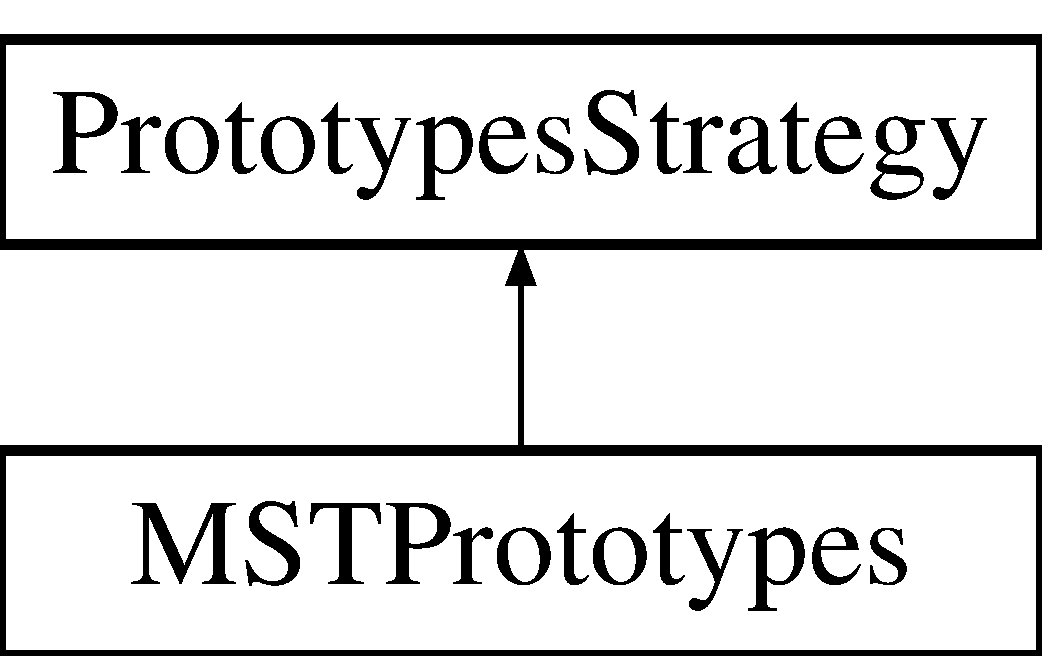
\includegraphics[height=2.000000cm]{classPrototypesStrategy}
\end{center}
\end{figure}
\subsection*{Public Member Functions}
\begin{DoxyCompactItemize}
\item 
virtual vector$<$ double $>$ \hyperlink{classPrototypesStrategy_a0422be14bb6be39a2d06112daf7043c1}{Select\+Prototypes} (\hyperlink{namespaceopf_a61631393754e0aa6aaeacf0767b2b419}{opf\+::\+Distance} distance, \hyperlink{classPatterns}{Patterns} patterns)=0
\begin{DoxyCompactList}\small\item\em Returns a vector with initial costs to all nodes. \end{DoxyCompactList}\end{DoxyCompactItemize}


\subsection{Detailed Description}
Strategy interface of way to select prototypes. 

All new strategy of selecting prototypes must implement this interface. \begin{DoxyAuthor}{Authors}
Alan Zanoni Peixinho \href{mailto:apeixinho@studends.ic.unicamp.br}{\tt apeixinho@studends.\+ic.\+unicamp.\+br} 

Luis Augusto Martins Pereria \href{mailto:lmartins@ic.unicamb.br}{\tt lmartins@ic.\+unicamb.\+br} 
\end{DoxyAuthor}
\begin{DoxyVersion}{Version}
1.\+0.\+0 
\end{DoxyVersion}


\subsection{Member Function Documentation}
\hypertarget{classPrototypesStrategy_a0422be14bb6be39a2d06112daf7043c1}{\index{Prototypes\+Strategy@{Prototypes\+Strategy}!Select\+Prototypes@{Select\+Prototypes}}
\index{Select\+Prototypes@{Select\+Prototypes}!Prototypes\+Strategy@{Prototypes\+Strategy}}
\subsubsection[{Select\+Prototypes}]{\setlength{\rightskip}{0pt plus 5cm}virtual vector$<$double$>$ Prototypes\+Strategy\+::\+Select\+Prototypes (
\begin{DoxyParamCaption}
\item[{{\bf opf\+::\+Distance}}]{distance, }
\item[{{\bf Patterns}}]{patterns}
\end{DoxyParamCaption}
)\hspace{0.3cm}{\ttfamily [pure virtual]}}}\label{classPrototypesStrategy_a0422be14bb6be39a2d06112daf7043c1}


Returns a vector with initial costs to all nodes. 

These costs are used to define roots/prototypes in the process of growing optimum-\/path trees during \hyperlink{classOPF}{O\+P\+F} training phase. 
\begin{DoxyParams}{Parameters}
{\em distance} & a similarity function. \\
\hline
{\em patterns} & set of input patterns. \\
\hline
\end{DoxyParams}
\begin{DoxySeeAlso}{See Also}
\hyperlink{classMSTPrototypes}{M\+S\+T\+Prototypes} 
\end{DoxySeeAlso}


Implemented in \hyperlink{classMSTPrototypes_a654ccbaebfdbca73a0da0e5eb1e4e39f}{M\+S\+T\+Prototypes}.



The documentation for this class was generated from the following file\+:\begin{DoxyCompactItemize}
\item 
Core/include/classifier/core/\hyperlink{prototypes__strategy_8h}{prototypes\+\_\+strategy.\+h}\end{DoxyCompactItemize}

\hypertarget{classTrainer}{\section{Trainer Class Reference}
\label{classTrainer}\index{Trainer@{Trainer}}
}


{\ttfamily \#include $<$trainer.\+h$>$}

\subsection*{Public Member Functions}
\begin{DoxyCompactItemize}
\item 
\hyperlink{classTrainer_ae46edcf554107399ffcd656ec7bd83ee}{Trainer} (opf\+::\+Distance distance, \hyperlink{classPrototypesStrategy}{Prototypes\+Strategy} prototypes, \hyperlink{classTrainingStrategy}{Training\+Strategy} trainer, \hyperlink{classPatterns}{Patterns} patterns)
\item 
virtual \hyperlink{classModel}{Model} \hyperlink{classTrainer_ade4ebb0af56d060829a8d86df0a1b11a}{train} ()
\end{DoxyCompactItemize}


\subsection{Constructor \& Destructor Documentation}
\hypertarget{classTrainer_ae46edcf554107399ffcd656ec7bd83ee}{\index{Trainer@{Trainer}!Trainer@{Trainer}}
\index{Trainer@{Trainer}!Trainer@{Trainer}}
\subsubsection[{Trainer}]{\setlength{\rightskip}{0pt plus 5cm}Trainer\+::\+Trainer (
\begin{DoxyParamCaption}
\item[{opf\+::\+Distance}]{distance, }
\item[{{\bf Prototypes\+Strategy}}]{prototypes, }
\item[{{\bf Training\+Strategy}}]{trainer, }
\item[{{\bf Patterns}}]{patterns}
\end{DoxyParamCaption}
)}}\label{classTrainer_ae46edcf554107399ffcd656ec7bd83ee}


\subsection{Member Function Documentation}
\hypertarget{classTrainer_ade4ebb0af56d060829a8d86df0a1b11a}{\index{Trainer@{Trainer}!train@{train}}
\index{train@{train}!Trainer@{Trainer}}
\subsubsection[{train}]{\setlength{\rightskip}{0pt plus 5cm}virtual {\bf Model} Trainer\+::train (
\begin{DoxyParamCaption}
{}
\end{DoxyParamCaption}
)\hspace{0.3cm}{\ttfamily [virtual]}}}\label{classTrainer_ade4ebb0af56d060829a8d86df0a1b11a}


The documentation for this class was generated from the following file\+:\begin{DoxyCompactItemize}
\item 
classifiers/includes/core/\hyperlink{trainer_8h}{trainer.\+h}\end{DoxyCompactItemize}

\hypertarget{classTrainingStrategy}{\section{Training\+Strategy Class Reference}
\label{classTrainingStrategy}\index{Training\+Strategy@{Training\+Strategy}}
}


Interface for training strategies.  




{\ttfamily \#include $<$training\+\_\+strategy.\+h$>$}

Inheritance diagram for Training\+Strategy\+:\begin{figure}[H]
\begin{center}
\leavevmode
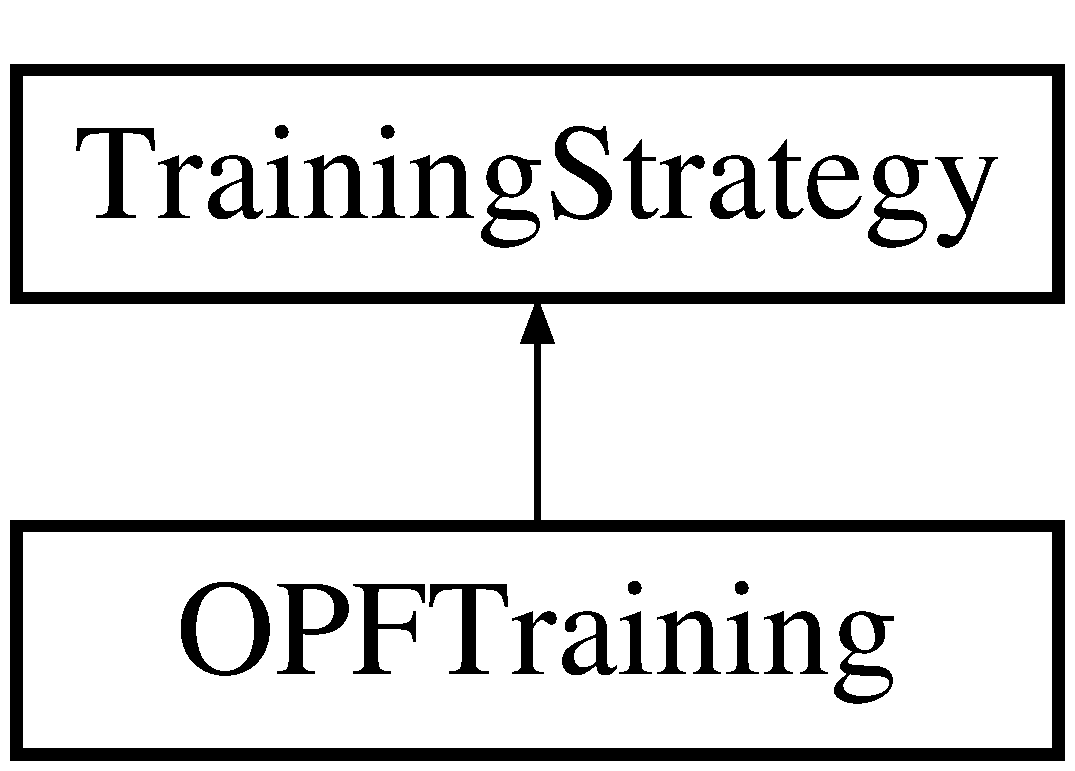
\includegraphics[height=2.000000cm]{classTrainingStrategy}
\end{center}
\end{figure}
\subsection*{Public Member Functions}
\begin{DoxyCompactItemize}
\item 
\hyperlink{classTrainingStrategy_ac52f574cc5540ea26115b5ee8f7b5c66}{Training\+Strategy} ()
\item 
virtual \hyperlink{classModel}{Model} $\ast$ \hyperlink{classTrainingStrategy_ad5da56b8b57e010c97a782d9e629e2b5}{train} ()
\end{DoxyCompactItemize}


\subsection{Detailed Description}
Interface for training strategies. 

One may want to develop a new \hyperlink{classOPF}{O\+P\+F} training strategy. Therefore, all new training strategy must implement this interface. 

\subsection{Constructor \& Destructor Documentation}
\hypertarget{classTrainingStrategy_ac52f574cc5540ea26115b5ee8f7b5c66}{\index{Training\+Strategy@{Training\+Strategy}!Training\+Strategy@{Training\+Strategy}}
\index{Training\+Strategy@{Training\+Strategy}!Training\+Strategy@{Training\+Strategy}}
\subsubsection[{Training\+Strategy}]{\setlength{\rightskip}{0pt plus 5cm}Training\+Strategy\+::\+Training\+Strategy (
\begin{DoxyParamCaption}
{}
\end{DoxyParamCaption}
)}}\label{classTrainingStrategy_ac52f574cc5540ea26115b5ee8f7b5c66}


\subsection{Member Function Documentation}
\hypertarget{classTrainingStrategy_ad5da56b8b57e010c97a782d9e629e2b5}{\index{Training\+Strategy@{Training\+Strategy}!train@{train}}
\index{train@{train}!Training\+Strategy@{Training\+Strategy}}
\subsubsection[{train}]{\setlength{\rightskip}{0pt plus 5cm}virtual {\bf Model}$\ast$ Training\+Strategy\+::train (
\begin{DoxyParamCaption}
{}
\end{DoxyParamCaption}
)\hspace{0.3cm}{\ttfamily [virtual]}}}\label{classTrainingStrategy_ad5da56b8b57e010c97a782d9e629e2b5}


The documentation for this class was generated from the following file\+:\begin{DoxyCompactItemize}
\item 
Core/include/classifier/core/\hyperlink{training__strategy_8h}{training\+\_\+strategy.\+h}\end{DoxyCompactItemize}

\chapter{File Documentation}
\hypertarget{main_8cpp}{\section{App/main.cpp File Reference}
\label{main_8cpp}\index{App/main.\+cpp@{App/main.\+cpp}}
}
{\ttfamily \#include $<$iostream$>$}\\*
{\ttfamily \#include $<$libopf-\/plus.\+h$>$}\\*
\subsection*{Functions}
\begin{DoxyCompactItemize}
\item 
int \hyperlink{main_8cpp_ae66f6b31b5ad750f1fe042a706a4e3d4}{main} ()
\end{DoxyCompactItemize}


\subsection{Function Documentation}
\hypertarget{main_8cpp_ae66f6b31b5ad750f1fe042a706a4e3d4}{\index{main.\+cpp@{main.\+cpp}!main@{main}}
\index{main@{main}!main.\+cpp@{main.\+cpp}}
\subsubsection[{main}]{\setlength{\rightskip}{0pt plus 5cm}int main (
\begin{DoxyParamCaption}
{}
\end{DoxyParamCaption}
)}}\label{main_8cpp_ae66f6b31b5ad750f1fe042a706a4e3d4}

\hypertarget{mst__prototype_8h}{\section{classifiers/includes/complete\+\_\+graph/mst\+\_\+prototype.h File Reference}
\label{mst__prototype_8h}\index{classifiers/includes/complete\+\_\+graph/mst\+\_\+prototype.\+h@{classifiers/includes/complete\+\_\+graph/mst\+\_\+prototype.\+h}}
}
{\ttfamily \#include \char`\"{}prototype\+\_\+strategy.\+h\char`\"{}}\\*
{\ttfamily \#include \char`\"{}utils/distance.\+h\char`\"{}}\\*
\subsection*{Classes}
\begin{DoxyCompactItemize}
\item 
class \hyperlink{classMSTPrototypes}{M\+S\+T\+Prototypes}
\end{DoxyCompactItemize}

\hypertarget{opf__classifying_8h}{\section{Core/include/classifier/complete\+\_\+graph/opf\+\_\+classifying.h File Reference}
\label{opf__classifying_8h}\index{Core/include/classifier/complete\+\_\+graph/opf\+\_\+classifying.\+h@{Core/include/classifier/complete\+\_\+graph/opf\+\_\+classifying.\+h}}
}
{\ttfamily \#include $<$classifier/core/classifying\+\_\+strategy.\+h$>$}\\*
{\ttfamily \#include $<$vector$>$}\\*
\subsection*{Classes}
\begin{DoxyCompactItemize}
\item 
class \hyperlink{classopf_1_1OPFClassifying}{opf\+::\+O\+P\+F\+Classifying}
\begin{DoxyCompactList}\small\item\em Class to handle prototypes selection by using a Minimum Spanning Tree (M\+S\+T). \end{DoxyCompactList}\end{DoxyCompactItemize}
\subsection*{Namespaces}
\begin{DoxyCompactItemize}
\item 
 \hyperlink{namespaceopf}{opf}
\begin{DoxyCompactList}\small\item\em Class for handling the training model informations. \end{DoxyCompactList}\end{DoxyCompactItemize}

\hypertarget{opf__training_8h}{\section{classifiers/includes/complete\+\_\+graph/opf\+\_\+training.h File Reference}
\label{opf__training_8h}\index{classifiers/includes/complete\+\_\+graph/opf\+\_\+training.\+h@{classifiers/includes/complete\+\_\+graph/opf\+\_\+training.\+h}}
}
\subsection*{Classes}
\begin{DoxyCompactItemize}
\item 
class \hyperlink{classOPFTraining}{O\+P\+F\+Training}
\end{DoxyCompactItemize}

\hypertarget{classifier_8h}{\section{classifiers/includes/core/classifier.h File Reference}
\label{classifier_8h}\index{classifiers/includes/core/classifier.\+h@{classifiers/includes/core/classifier.\+h}}
}
{\ttfamily \#include \char`\"{}utils/distance.\+h\char`\"{}}\\*
\subsection*{Classes}
\begin{DoxyCompactItemize}
\item 
class \hyperlink{classClassifier}{Classifier}
\end{DoxyCompactItemize}

\hypertarget{classifying__strategy_8h}{\section{classifiers/includes/core/classifying\+\_\+strategy.h File Reference}
\label{classifying__strategy_8h}\index{classifiers/includes/core/classifying\+\_\+strategy.\+h@{classifiers/includes/core/classifying\+\_\+strategy.\+h}}
}
\subsection*{Classes}
\begin{DoxyCompactItemize}
\item 
class \hyperlink{classClassifyingStrategy}{Classifying\+Strategy}
\end{DoxyCompactItemize}

\hypertarget{model_8h}{\section{Core/include/classifier/core/model.h File Reference}
\label{model_8h}\index{Core/include/classifier/core/model.\+h@{Core/include/classifier/core/model.\+h}}
}
{\ttfamily \#include $<$classifier/core/model\+\_\+node.\+h$>$}\\*
{\ttfamily \#include $<$input/patterns.\+h$>$}\\*
{\ttfamily \#include $<$utils/distance.\+h$>$}\\*
\subsection*{Classes}
\begin{DoxyCompactItemize}
\item 
class \hyperlink{classopf_1_1Model}{opf\+::\+Model}
\end{DoxyCompactItemize}
\subsection*{Namespaces}
\begin{DoxyCompactItemize}
\item 
 \hyperlink{namespaceopf}{opf}
\begin{DoxyCompactList}\small\item\em Class for handling the training model informations. \end{DoxyCompactList}\end{DoxyCompactItemize}

\hypertarget{model__node_8h}{\section{Core/include/classifier/core/model\+\_\+node.h File Reference}
\label{model__node_8h}\index{Core/include/classifier/core/model\+\_\+node.\+h@{Core/include/classifier/core/model\+\_\+node.\+h}}
}
{\ttfamily \#include $<$input/pattern.\+h$>$}\\*

\hypertarget{opf_8h}{\section{classifiers/includes/core/opf.h File Reference}
\label{opf_8h}\index{classifiers/includes/core/opf.\+h@{classifiers/includes/core/opf.\+h}}
}
{\ttfamily \#include \char`\"{}training/model.\+h\char`\"{}}\\*
{\ttfamily \#include \char`\"{}training/trainer.\+h\char`\"{}}\\*
{\ttfamily \#include \char`\"{}utils/distance.\+h\char`\"{}}\\*
\subsection*{Classes}
\begin{DoxyCompactItemize}
\item 
class \hyperlink{classOPF}{O\+P\+F}
\end{DoxyCompactItemize}

\hypertarget{prototype__strategy_8h}{\section{Core/include/classifier/core/prototype\+\_\+strategy.h File Reference}
\label{prototype__strategy_8h}\index{Core/include/classifier/core/prototype\+\_\+strategy.\+h@{Core/include/classifier/core/prototype\+\_\+strategy.\+h}}
}
{\ttfamily \#include $<$input/pattern.\+h$>$}\\*
{\ttfamily \#include $<$input/patterns.\+h$>$}\\*
{\ttfamily \#include $<$utils/distance.\+h$>$}\\*
{\ttfamily \#include $<$libopf-\/plus.\+h$>$}\\*
{\ttfamily \#include $<$vector$>$}\\*
\subsection*{Classes}
\begin{DoxyCompactItemize}
\item 
class \hyperlink{classPrototypesStrategy}{Prototypes\+Strategy}
\begin{DoxyCompactList}\small\item\em Strategy interface of way to select prototypes. \end{DoxyCompactList}\end{DoxyCompactItemize}

\hypertarget{trainer_8h}{\section{Core/include/classifier/core/trainer.h File Reference}
\label{trainer_8h}\index{Core/include/classifier/core/trainer.\+h@{Core/include/classifier/core/trainer.\+h}}
}
{\ttfamily \#include $<$utils/distance.\+h$>$}\\*
{\ttfamily \#include $<$classifier/core/prototypes\+\_\+strategy.\+h$>$}\\*
{\ttfamily \#include $<$classifier/core/training\+\_\+strategy.\+h$>$}\\*
\subsection*{Classes}
\begin{DoxyCompactItemize}
\item 
class \hyperlink{classTrainer}{Trainer}
\end{DoxyCompactItemize}

\hypertarget{training__strategy_8h}{\section{Core/include/classifier/core/training\+\_\+strategy.h File Reference}
\label{training__strategy_8h}\index{Core/include/classifier/core/training\+\_\+strategy.\+h@{Core/include/classifier/core/training\+\_\+strategy.\+h}}
}
{\ttfamily \#include $<$classifier/core/model.\+h$>$}\\*
\subsection*{Classes}
\begin{DoxyCompactItemize}
\item 
class \hyperlink{classTrainingStrategy}{Training\+Strategy}
\begin{DoxyCompactList}\small\item\em Interface for training strategies. \end{DoxyCompactList}\end{DoxyCompactItemize}

\hypertarget{file__formats_8h}{\section{Core/include/input/file\+\_\+formats.h File Reference}
\label{file__formats_8h}\index{Core/include/input/file\+\_\+formats.\+h@{Core/include/input/file\+\_\+formats.\+h}}
}
{\ttfamily \#include $<$iostream$>$}\\*
{\ttfamily \#include $<$input/patterns.\+h$>$}\\*
\subsection*{Classes}
\begin{DoxyCompactItemize}
\item 
class \hyperlink{classCsvAdapter}{Csv\+Adapter}
\end{DoxyCompactItemize}

\hypertarget{pattern_8h}{\section{Core/include/input/pattern.h File Reference}
\label{pattern_8h}\index{Core/include/input/pattern.\+h@{Core/include/input/pattern.\+h}}
}
{\ttfamily \#include $<$istream$>$}\\*
{\ttfamily \#include $<$iterator$>$}\\*
{\ttfamily \#include $<$vector$>$}\\*
{\ttfamily \#include $<$iostream$>$}\\*
\subsection*{Classes}
\begin{DoxyCompactItemize}
\item 
class \hyperlink{classopf_1_1Pattern}{opf\+::\+Pattern}
\begin{DoxyCompactList}\small\item\em Class for handling a single pattern. \end{DoxyCompactList}\end{DoxyCompactItemize}
\subsection*{Namespaces}
\begin{DoxyCompactItemize}
\item 
 \hyperlink{namespaceopf}{opf}
\begin{DoxyCompactList}\small\item\em Class for handling the training model informations. \end{DoxyCompactList}\end{DoxyCompactItemize}

\hypertarget{patterns_8h}{\section{input/includes/patterns.h File Reference}
\label{patterns_8h}\index{input/includes/patterns.\+h@{input/includes/patterns.\+h}}
}
{\ttfamily \#include $<$string$>$}\\*
{\ttfamily \#include $<$iostream$>$}\\*
{\ttfamily \#include $<$fstream$>$}\\*
{\ttfamily \#include $<$stdlib.\+h$>$}\\*
{\ttfamily \#include \char`\"{}pattern.\+h\char`\"{}}\\*
\subsection*{Classes}
\begin{DoxyCompactItemize}
\item 
class \hyperlink{classPatterns}{Patterns}
\end{DoxyCompactItemize}

\hypertarget{libopf-plus_8h}{\section{Core/include/libopf-\/plus.h File Reference}
\label{libopf-plus_8h}\index{Core/include/libopf-\/plus.\+h@{Core/include/libopf-\/plus.\+h}}
}
{\ttfamily \#include $<$classifier/core/opf.\+h$>$}\\*
{\ttfamily \#include $<$classifier/core/model.\+h$>$}\\*
{\ttfamily \#include $<$utils/distance.\+h$>$}\\*
{\ttfamily \#include $<$input/file\+\_\+formats.\+h$>$}\\*
{\ttfamily \#include $<$utils/priority\+\_\+queue.\+h$>$}\\*

\hypertarget{distance_8h}{\section{Core/include/utils/distance.h File Reference}
\label{distance_8h}\index{Core/include/utils/distance.\+h@{Core/include/utils/distance.\+h}}
}
{\ttfamily \#include $<$functional$>$}\\*
{\ttfamily \#include $<$vector$>$}\\*
\subsection*{Namespaces}
\begin{DoxyCompactItemize}
\item 
 \hyperlink{namespaceopf}{opf}
\begin{DoxyCompactList}\small\item\em Class for handling the training model informations. \end{DoxyCompactList}\end{DoxyCompactItemize}
\subsection*{Typedefs}
\begin{DoxyCompactItemize}
\item 
typedef std\+::function$<$ double(const \\*
vector$<$ double $>$, const vector\\*
$<$ double $>$)$>$ \hyperlink{namespaceopf_a61631393754e0aa6aaeacf0767b2b419}{opf\+::\+Distance}
\end{DoxyCompactItemize}

\hypertarget{priority__queue_8h}{\section{Core/include/utils/priority\+\_\+queue.h File Reference}
\label{priority__queue_8h}\index{Core/include/utils/priority\+\_\+queue.\+h@{Core/include/utils/priority\+\_\+queue.\+h}}
}
{\ttfamily \#include $<$vector$>$}\\*
{\ttfamily \#include $<$iterator$>$}\\*
{\ttfamily \#include $<$functional$>$}\\*
{\ttfamily \#include $<$limits$>$}\\*
{\ttfamily \#include $<$utils/queue\+\_\+element.\+h$>$}\\*
\subsection*{Classes}
\begin{DoxyCompactItemize}
\item 
class \hyperlink{classopf_1_1PriorityQueue}{opf\+::\+Priority\+Queue}
\begin{DoxyCompactList}\small\item\em Class for handling minimum and maximum priority queues. \end{DoxyCompactList}\end{DoxyCompactItemize}
\subsection*{Namespaces}
\begin{DoxyCompactItemize}
\item 
 \hyperlink{namespaceopf}{opf}
\begin{DoxyCompactList}\small\item\em Class for handling the training model informations. \end{DoxyCompactList}\end{DoxyCompactItemize}

\hypertarget{mst__prototype_8cpp}{\section{classifiers/src/complete\+\_\+graph/src/mst\+\_\+prototype.cpp File Reference}
\label{mst__prototype_8cpp}\index{classifiers/src/complete\+\_\+graph/src/mst\+\_\+prototype.\+cpp@{classifiers/src/complete\+\_\+graph/src/mst\+\_\+prototype.\+cpp}}
}
{\ttfamily \#include \char`\"{}mst\+\_\+prototype.\+h\char`\"{}}\\*
{\ttfamily \#include \char`\"{}prototypes\+\_\+strategy.\+h\char`\"{}}\\*
{\ttfamily \#include $<$utility$>$}\\*

\hypertarget{opf__classifying_8cpp}{\section{Core/src/classifier/complete\+\_\+graph/opf\+\_\+classifying.cpp File Reference}
\label{opf__classifying_8cpp}\index{Core/src/classifier/complete\+\_\+graph/opf\+\_\+classifying.\+cpp@{Core/src/classifier/complete\+\_\+graph/opf\+\_\+classifying.\+cpp}}
}
{\ttfamily \#include $<$classifier/complete\+\_\+graph/opf\+\_\+classifying.\+h$>$}\\*
{\ttfamily \#include $<$classifier/core/model.\+h$>$}\\*

\hypertarget{opf__training_8cpp}{\section{Core/src/classifier/complete\+\_\+graph/opf\+\_\+training.cpp File Reference}
\label{opf__training_8cpp}\index{Core/src/classifier/complete\+\_\+graph/opf\+\_\+training.\+cpp@{Core/src/classifier/complete\+\_\+graph/opf\+\_\+training.\+cpp}}
}
{\ttfamily \#include $<$classifier/complete\+\_\+graph/opf\+\_\+training.\+h$>$}\\*
{\ttfamily \#include $<$classifier/complete\+\_\+graph/mst\+\_\+prototype.\+h$>$}\\*
{\ttfamily \#include $<$classifier/core/model.\+h$>$}\\*
{\ttfamily \#include $<$libopf-\/plus.\+h$>$}\\*

\hypertarget{model_8cpp}{\section{Core/src/classifier/core/model.cpp File Reference}
\label{model_8cpp}\index{Core/src/classifier/core/model.\+cpp@{Core/src/classifier/core/model.\+cpp}}
}
{\ttfamily \#include $<$classifier/core/model.\+h$>$}\\*
{\ttfamily \#include $<$libopf-\/plus.\+h$>$}\\*

\hypertarget{model__node_8cpp}{\section{Core/src/classifier/core/model\+\_\+node.cpp File Reference}
\label{model__node_8cpp}\index{Core/src/classifier/core/model\+\_\+node.\+cpp@{Core/src/classifier/core/model\+\_\+node.\+cpp}}
}
{\ttfamily \#include $<$classifier/core/model\+\_\+node.\+h$>$}\\*

\hypertarget{opf_8cpp}{\section{Core/src/classifier/core/opf.cpp File Reference}
\label{opf_8cpp}\index{Core/src/classifier/core/opf.\+cpp@{Core/src/classifier/core/opf.\+cpp}}
}
{\ttfamily \#include $<$classifier/core/opf.\+h$>$}\\*

\hypertarget{file__formats_8cpp}{\section{Core/src/input/file\+\_\+formats.cpp File Reference}
\label{file__formats_8cpp}\index{Core/src/input/file\+\_\+formats.\+cpp@{Core/src/input/file\+\_\+formats.\+cpp}}
}
{\ttfamily \#include $<$input/file\+\_\+formats.\+h$>$}\\*
\subsection*{Functions}
\begin{DoxyCompactItemize}
\item 
istream \& \hyperlink{file__formats_8cpp_a2a2e2f128a329757f385bbd6d0d3f0b4}{operator$>$$>$} (istream \&in, Csv\+Adapter \&c)
\end{DoxyCompactItemize}


\subsection{Function Documentation}
\hypertarget{file__formats_8cpp_a2a2e2f128a329757f385bbd6d0d3f0b4}{\index{file\+\_\+formats.\+cpp@{file\+\_\+formats.\+cpp}!operator$>$$>$@{operator$>$$>$}}
\index{operator$>$$>$@{operator$>$$>$}!file\+\_\+formats.\+cpp@{file\+\_\+formats.\+cpp}}
\subsubsection[{operator$>$$>$}]{\setlength{\rightskip}{0pt plus 5cm}istream\& operator$>$$>$ (
\begin{DoxyParamCaption}
\item[{istream \&}]{in, }
\item[{Csv\+Adapter \&}]{c}
\end{DoxyParamCaption}
)}}\label{file__formats_8cpp_a2a2e2f128a329757f385bbd6d0d3f0b4}

\hypertarget{pattern_8cpp}{\section{Core/src/input/pattern.cpp File Reference}
\label{pattern_8cpp}\index{Core/src/input/pattern.\+cpp@{Core/src/input/pattern.\+cpp}}
}
{\ttfamily \#include $<$input/pattern.\+h$>$}\\*
{\ttfamily \#include $<$iostream$>$}\\*
{\ttfamily \#include $<$assert.\+h$>$}\\*
\subsection*{Namespaces}
\begin{DoxyCompactItemize}
\item 
 \hyperlink{namespaceopf}{opf}
\begin{DoxyCompactList}\small\item\em Class for handling the training model informations. \end{DoxyCompactList}\end{DoxyCompactItemize}
\subsection*{Functions}
\begin{DoxyCompactItemize}
\item 
ostream \& \hyperlink{namespaceopf_acf5fd15fc266cd630fe92b43dcdf8d21}{opf\+::operator$<$$<$} (ostream \&output, const Pattern \&pattern)
\item 
istream \& \hyperlink{namespaceopf_a982afea1c95e9fb04a185a92c32365ac}{opf\+::operator$>$$>$} (istream \&in, Pattern \&pattern)
\end{DoxyCompactItemize}

\hypertarget{patterns_8cpp}{\section{Core/src/input/patterns.cpp File Reference}
\label{patterns_8cpp}\index{Core/src/input/patterns.\+cpp@{Core/src/input/patterns.\+cpp}}
}
{\ttfamily \#include $<$input/patterns.\+h$>$}\\*
{\ttfamily \#include $<$input/pattern.\+h$>$}\\*
\subsection*{Functions}
\begin{DoxyCompactItemize}
\item 
istream \& \hyperlink{patterns_8cpp_aed3f40599aaf63a1f5126b3acac33fb4}{operator$>$$>$} (istream \&input, \hyperlink{classPatterns}{Patterns} \&patterns)
\end{DoxyCompactItemize}


\subsection{Function Documentation}
\hypertarget{patterns_8cpp_aed3f40599aaf63a1f5126b3acac33fb4}{\index{patterns.\+cpp@{patterns.\+cpp}!operator$>$$>$@{operator$>$$>$}}
\index{operator$>$$>$@{operator$>$$>$}!patterns.\+cpp@{patterns.\+cpp}}
\subsubsection[{operator$>$$>$}]{\setlength{\rightskip}{0pt plus 5cm}istream\& operator$>$$>$ (
\begin{DoxyParamCaption}
\item[{istream \&}]{input, }
\item[{{\bf Patterns} \&}]{patterns}
\end{DoxyParamCaption}
)}}\label{patterns_8cpp_aed3f40599aaf63a1f5126b3acac33fb4}

\hypertarget{priority__queue_8cpp}{\section{Core/src/utils/priority\+\_\+queue.cpp File Reference}
\label{priority__queue_8cpp}\index{Core/src/utils/priority\+\_\+queue.\+cpp@{Core/src/utils/priority\+\_\+queue.\+cpp}}
}
{\ttfamily \#include $<$utils/priority\+\_\+queue.\+h$>$}\\*
{\ttfamily \#include $<$limits$>$}\\*
{\ttfamily \#include $<$algorithm$>$}\\*
{\ttfamily \#include $<$functional$>$}\\*
{\ttfamily \#include $<$iterator$>$}\\*
{\ttfamily \#include $<$exception/opf\+\_\+exception.\+h$>$}\\*

\hypertarget{README_8md}{\section{R\+E\+A\+D\+M\+E.\+md File Reference}
\label{README_8md}\index{R\+E\+A\+D\+M\+E.\+md@{R\+E\+A\+D\+M\+E.\+md}}
}

%--- End generated contents ---

% Index
\newpage
\phantomsection
\addcontentsline{toc}{chapter}{Index}
\printindex

\end{document}
